\documentclass[conference]{IEEEtran}

\usepackage[UTF8,scheme=plain]{ctex}
\usepackage{amsmath,amssymb}
\usepackage{booktabs}
\usepackage{graphicx}
\usepackage{array}
\usepackage{url}

\newcommand{\missingfigure}[1]{%
  \fbox{\parbox[c][3.8cm][c]{0.92\textwidth}{\centering #1}}%
}

\title{基于正常模板与多模态大模型的 PCB 缺陷检测结果复核方法\\
{\large Reference-Guided Multimodal Verification for PCB Defect Detection}}
\author{\IEEEauthorblockN{匿名作者}}

\begin{document}
\maketitle

\begin{abstract}
针对 PCB 表面缺陷检测器在细粒度线路变化、正常纹理扰动和相似缺陷类别下出现的误报、
漏检与错分类问题，本文提出一种基于正常模板与多模态大模型的检测结果复核方法。
方法联合基础检测器的语义候选与正常模板的差异候选构建统一候选集合，
使系统既能复核已有检测结果，也能验证检测器未提出的潜在漏检区域；
在此基础上由学习式复检门控制大模型的调用预算，
由外部证据驱动的接受门约束修改动作是否执行。
在 DeepPCB 上按模板组隔离的五折交叉验证表明，
基础检测器留下 1644 个可纠错错误，其中漏检占 57.6\%。
不加门控时大模型复检的有害修正率达到 0.9326，最终 F1 由 0.9118 降至 0.8660；
引入双门控后正确检测保留率为 0.9998，最终 F1 与基础检测器无统计差异。
复检门在 5\% 调用预算下定位 46.5\% 的可纠错错误，随机策略仅为 3.2\%。
证据消融显示正常模板是唯一稳定的增益来源，
而外观差异图与拓扑差异图作为大模型视觉输入未带来增益。
接受上界分析进一步表明，即使完美采纳大模型的全部提议，
最终 F1 也仅比基础检测器高 0.0025，
说明当前多模态大模型在工业细粒度缺陷验证上的判断质量是系统的主要瓶颈。
\end{abstract}

\begin{IEEEkeywords}
PCB 缺陷检测，检测结果复核，正常模板参照，多模态大模型，选择性预测，风险门控
\end{IEEEkeywords}

\section{绪论}
\label{sec:introduction}

印制电路板（Printed Circuit Board，PCB）承载电子器件，并负责电气连接与信号传输。线路开路、短路、鼠咬、毛刺、针孔和多余铜等表面缺陷会改变局部导通状态。这些缺陷还会在后续装配与服役阶段引发间歇性故障。线路密度和制造节拍提高后，人工逐板检查难以兼顾一致性、速度与成本。自动光学检测（Automated Optical Inspection，AOI）已成为 PCB 制造质量控制的常用环节。其典型流程先快速定位疑似区域，再由规则、模型或操作员复判报警是否成立\cite{deng2018autovrs,chen2023pcbreview}。误报会增加停线和人工确认成本，漏检会使结构性缺陷进入后续工序。复核系统因此需要同时评价纠错收益、正确结果保护与处理开销。

基于卷积神经网络和视觉 Transformer 的目标检测器提高了 PCB 缺陷定位的自动化程度\cite{tang2019deeppcb,chen2023pcbreview}。这类方法通常以待检图像为主要输入，通过多尺度特征识别局部纹理异常。单图检测仍有结构性局限。PCB 缺陷往往只占几十个像素，细小目标容易在下采样过程中丢失。正常线路的局部纹理重复、密集且高度相似，灰尘、反光和轻微成像偏差也会产生类似缺陷的响应。开路与短路的判别依据并非普通物体的外观语义，而是线路是否保持应有的连通、隔离和分支关系。仅凭当前图像，系统难以稳定区分多余铜、正常焊盘与光照扰动。叠加检测头、注意力模块或损失项可以改善特征表达，但无法补充同位置的正常状态。

正常模板为这些问题提供了反事实参照。单图检测器回答“该区域是否像缺陷”，模板比较则回答“该位置相对正常设计发生了什么变化”。对于开路，正常模板给出本应连续的铜线；对于短路，正常模板给出本应隔离的线路。对于鼠咬、毛刺、针孔和多余铜，正常模板分别给出完整边缘、正常轮廓、孔结构及铜区范围。配对正常模板使变化判断受到正常结构约束。已有 PCB 检测和工业变化检测工作表明模板信息具有应用价值\cite{tang2019deeppcb,fridman2021changechip}。模板差分仍会受到配准误差、光度变化和阈值噪声影响，因此差异区域只用于提出待验证假设，不能直接视为真实缺陷。

本文将多模态大模型（Multimodal Large Language Model，MLLM）简称为 MLLM。MLLM 能够联合处理局部图像、正常模板和封闭缺陷定义\cite{jiang2025mmad,xu2025anomalyov,andrade2026agreementbias}。与固定阈值规则相比，MLLM 可以组合多种视觉线索，并在预先限定的类别空间内输出结构化判断。通用 MLLM 对极小异常的感知能力有限，也会依赖文字先验或生成不存在的结构。其自报置信度不能直接作为工业决策依据。让 MLLM 在整幅 PCB 图像上自由定位会增加调用成本，并引入不受约束的新框。把基础检测器的类别和置信度直接写入提示，则会产生既有答案锚定风险。因此，本文把 MLLM 限定为局部、选择性、可审计且受安全规则约束的多模态验证器。

本文研究挂接在基础检测器之后的 PCB 缺陷结果复核。系统将检测候选与正常模板差异模块产生的差异候选合并为统一候选空间。多模态验证器只判断已有候选，不在任意位置生成新框。复核调用选择门（简称复检门）从中选择需要调用 MLLM 的高风险候选，接受门再判断提议动作是否有足够的外部证据。前者控制调用效率，后者约束修改风险。最终系统使用 A2 三面板证据卡，包括当前紧裁剪、正常模板紧裁剪和更大上下文。外观差异图与拓扑差异图不作为 MLLM 的视觉输入，拓扑向量仅用于门控决策。系统设计和实验评价均明确考察 MLLM 的能力边界。

本文的贡献包括以下三点。

\begin{enumerate}
  \item \textbf{面向漏检恢复的双来源候选机制。}该机制联合检测候选与差异候选，在统一候选空间中处理误报、错分类和检测器未提出候选的漏检。差异候选的漏检恢复候选率为 0.625（IoU 0.3）。候选上界 F1 为 0.9555，相对基线 0.9118 留有 $+0.044$ 空间，表明候选覆盖并非主要限制因素。五折错误分解中，漏检占可纠错空间的 57.6\%，在三类错误中占比最高。

  \item \textbf{风险受控的分级复核机制。}学习式复检门控制调用预算，外部证据驱动的接受门约束修改动作。复检门在 5\% 调用预算下定位 46.5\% 的可纠错错误，随机策略为 3.2\%，前者是后者的 14.8 倍。有接受门的预算曲线 F1 为 0.9115 至 0.9117，与基线 0.9118 无统计差异；无接受门时，F1 随预算从 0.9088 降至 0.8660。双门控的正确检测保留率为 0.9998，734 个正确检测中误删 2 个。双门控还将有害修正率从无门控时的 0.9326 降至 0.4000，并把误删控制在 2 次。

  \item \textbf{MLLM 作为工业细粒度缺陷验证器的能力边界实证。}正常模板是证据消融中唯一稳定的增益来源。A2 相对 A0 提升 0.1178，置信区间不跨 0。阶段 C 的 200 候选主消融中，A4 的 F1 为 0.7571，略高于 A2 的 0.7553，但该差异在置信区间内，未证明拓扑图带来增量。阶段 B2 的 450 次专门对照中，A2 的 F1 为 0.8082，高于全部含差异图的变体。对渲染自动拉伸与配准残差的排查没有改变这一结论。Oracle 分析显示，候选上界为 0.9555，接受上界为 0.9143，仅比基线高 0.0025。主要限制来自 MLLM 提议动作中正确项不足。附加对照还显示，去锚定未见收益，配准不可靠提示产生负效应，自由文本输出的 JSON 可解析率为 0。
\end{enumerate}

第~\ref{sec:related} 节梳理 PCB 缺陷检测、正常模板比较、工业异常多模态理解及选择性决策研究。第~\ref{sec:problem} 节定义双来源候选、六种复核动作及整体数据流。第~\ref{sec:candidates} 节介绍模板处理、差异候选生成、候选融合和三面板证据卡。第~\ref{sec:gating} 节说明复检门、多模态验证器、动作映射、接受门和最终融合。第~\ref{sec:experiments} 节报告实验设置、证据消融、端到端纠错、预算曲线与鲁棒性分析。第~\ref{sec:conclusion} 节总结研究结论、局限和后续方向。

\section{相关工作}
\label{sec:related}

\subsection{PCB 缺陷检测与公开数据集}

公开数据集推动了 PCB 缺陷检测从手工规则向数据驱动方法转变。DeepPCB 包含 1500 对已配准的正常模板与待检图像，并标注六类常见裸板缺陷。其原始检测器直接以图像对为输入\cite{tang2019deeppcb}。Huang 和 Wei 发布的数据集包含 10 个模板和 1386 张合成缺陷图像。该数据集还提供检测、分类与配准任务所需信息\cite{huang2019hripcb}。这两类数据均保留配对正常模板，适合研究配对比较，但图像规模和缺陷生成方式与真实产线仍有差距。

面向真实制造条件的数据集补充了更多场景。DsPCBSD+ 收集产线 AOI 图像，并按缺陷成因、位置与形态细分类型\cite{lv2024dspcbsd}。PCB-IND 保留工业成像中的非均匀照明、长尾分布和跨尺度缺陷\cite{yan2026pcbind}。工业异常检测数据集 VisA 覆盖 12 类对象，并提供图像级与像素级标注，其中包含 PCB 类别\cite{zou2022visa}。这些数据扩大了场景多样性，但并非都为每张待检图提供严格对应的正常模板。本文的主要实验基于 DeepPCB 的配对结构，结论不外推到跨模板或跨产线场景。

\subsection{正常模板比较与变化检测}

正常模板参与的 PCB 检测并非新的问题设定。DeepPCB 联合编码正常模板和待检图，通过组金字塔池化预测缺陷\cite{tang2019deeppcb}。Auto-VRS 在 AOI 之后执行快速电路比较，再用深度网络判断候选是真缺陷还是伪缺陷，形成后置验证流程\cite{deng2018autovrs}。CSS-Net 使用标准板作为正常模板，与候选图像构成孪生输入。该方法以代价敏感阈值减少真实缺陷被判为伪缺陷的风险\cite{miao2021cssnet}。这些工作说明，检测后复核和正常模板二次分类本身不能构成本文的独立创新。

ChangeChip 将作为正常模板的 golden PCB 与待检板配准，再以无监督变化检测得到的变化区域提示缺陷\cite{fridman2021changechip}。RefDiffNet 在检测器主干之前加入轻量参考比较模块，将结构变化编码为增强后的检测输入。该方法在 DeepPCB 与 HRIPCB 上测试了模块的可插拔性\cite{edula2026refdiffnet}。这些工作分别代表独立变化检测和检测前参考增强。本文采用检测器后置复核：基础检测器先产生检测候选，差异候选补充漏检假设。多模态验证器只判断候选，接受门决定是否修改基础输出。外观差异图与拓扑图作为视觉证据未证明相对 A2 的稳定增量，最终系统已移除这两类视觉输入。

\subsection{工业异常检测中的多模态大模型}

AnomalyGPT 通过异常数据构造、视觉解码器和提示学习增强 MLLM 对局部工业异常的感知\cite{gu2024anomalygpt}。VMAD 将视觉异常知识和细粒度局部特征注入 MLLM，用于零样本检测、定位与解释\cite{deng2024vmad}。EMIT 采用面向困难样本的 GRPO 训练，以领域数据和热图引导工业异常识别\cite{guan2025emit}。这类方法主要改造模型本体，说明通用 MLLM 对微小工业异常的视觉能力仍需专门适配。

基准研究直接报告了 MLLM 的能力边界。MMAD 将工业异常检查拆分为识别、分类、定位、描述和分析等子任务，并指出现有 MLLM 与工业要求之间仍有差距\cite{jiang2025mmad}。Anomaly-OV 通过异常视觉 token 和特征匹配强化细粒度异常感知\cite{xu2025anomalyov}。UniPCB 面向开放式 PCB 质量检查构建统一视觉语言基准，并报告通用模型在领域任务上的不足\cite{sun2026unipcb}。DifferAD-R1 采用正常模板与待检图的双图差异引导，将工业异常定位表述为差异 grounding 问题\cite{wang2026differadr1}。“正常模板加 MLLM”因此也不属于本文的创新边界。本文把 MLLM 放在已有检测器之后，由复检门控制调用。接受门和安全规则约束修改，研究对象是复核系统的成本与风险，而非新的异常感知模型。

\subsection{选择性预测、校准与验证器可靠性}

复核系统需要同时回答“哪些候选值得调用昂贵模型”和“模型给出的修改能否执行”。SelectiveNet 将拒识机制与预测器联合训练，以风险和覆盖率描述选择性预测\cite{geifman2019selectivenet}。温度缩放使用单一参数校准神经网络置信度，为检测器工作点和门控特征提供了简单基线\cite{guo2017calibration}。Learning to Defer 学习把样本交给下游专家的条件，并把系统性能而非单一模型精度作为优化对象\cite{mozannar2020defer}。Conformal Risk Control 则把共形方法扩展到单调损失的期望风险控制\cite{angelopoulos2024conformalrisk}。这些研究共同表明，覆盖率、风险和校准应当分开报告，模型的高置信度不能直接等同于动作安全。

将 MLLM 用作多模态验证器还会引入新的偏差。研究发现，MLLM 会过度认可给定行为或既有答案，即同意偏差。先形成独立先验再验证候选可以缓解该问题\cite{andrade2026agreementbias}。自我修正综述指出，在缺少可靠外部反馈时，仅依赖模型自评不能稳定改正错误\cite{kamoi2024selfcorrection}。MLLM 的选择性预测研究也显示，外部视觉与几何信号比模型自报置信度更有判别力\cite{imran2026trustvlm}。本文不直接执行 MLLM 输出。接受门结合候选来源、配准质量、检测置信度和动作类型进行系统侧决策，硬安全规则保护已有正确检测。

\subsection{本文定位与差异化矩阵}

表~\ref{tab:positioning} 按实验结论界定本文位置。符号“有”只表示对应机制在该工作中明确出现，不将检测前增强、独立异常定位或开放式问答视为检测器后置修正。本文保留配对正常模板、差异候选和配准可靠性信号。显式差异视觉输入未证明相对 A2 的增量，因此已从最终系统中移除。

\begin{table*}[t]
  \centering
  \caption{相关方法与本文最终系统的差异化定位}
  \label{tab:positioning}
  \scriptsize
  \setlength{\tabcolsep}{3.2pt}
  \renewcommand{\arraystretch}{1.18}
  \begin{tabular}{lcccccccc}
    \hline
    方法 & 配对正常模板 & 显式差异证据 & 多模态验证 & 后置修正检测器 & 差异候选恢复漏检 & 配准质量阈值 & 复检门 & 接受门与安全规则 \\
    \hline
    DeepPCB\cite{tang2019deeppcb} & 有 & 无 & 无 & 无 & 无 & 无 & 无 & 无 \\
    Auto-VRS\cite{deng2018autovrs} & 有 & 有 & 无 & 有 & 无 & 无 & 无 & 无 \\
    CSS-Net\cite{miao2021cssnet} & 有 & 无 & 无 & 有 & 无 & 无 & 无 & 无 \\
    ChangeChip\cite{fridman2021changechip} & 有 & 有 & 无 & 无 & 无 & 部分 & 无 & 无 \\
    RefDiffNet\cite{edula2026refdiffnet} & 有 & 有 & 无 & 检测前增强 & 无 & 无 & 无 & 无 \\
    UniPCB\cite{sun2026unipcb} & 部分任务 & 可选 & 检测与问答 & 无 & 无 & 无 & 无 & 无 \\
    DifferAD-R1\cite{wang2026differadr1} & 有 & 有 & 定位 & 无 & 无 & 无 & 无 & 无 \\
    \textbf{本文} & 有 & \textbf{未证明增量，已移除} & 有 & 有 & 有 & 有 & 有 & 有 \\
    \hline
  \end{tabular}
\end{table*}

本文不主张首次使用正常模板、差异图或 MLLM 复核。差异化来自三个可检验的系统机制：检测候选与差异候选形成双来源互补；复检门控制有限调用预算；接受门与安全规则约束 MLLM 的修改动作。实验同时给出适用边界。正常模板是稳定的视觉增益来源，显式外观与拓扑证据未证明稳定增量，去锚定输入也未显示优势。

\section{问题定义与总体框架}
\label{sec:problem}

\subsection{任务定义}

本文研究 PCB 基础检测结果的候选级复核。系统读取待检图像 $I$、对应的正常模板 $R$ 和基础检测器 $D$。其余输入为封闭缺陷知识集合 $K$ 与多模态验证器 $V$。系统在有限验证预算下修正误报、漏检与错分类，并以正确检测保留率约束对已有正确结果的破坏。知识集合 $K$ 只包含系统允许识别的缺陷类别、类别定义和结构化输出约束。验证器 $V$ 读取候选的局部证据与 $K$，独立判断缺陷存在性和类别。它不是全图检测器，也不直接决定最终检测集合。

基础检测器在待检图像上产生检测候选集合
\begin{equation}
  C_{\mathrm{det}}=D(I)=\{(b_i,c_i,p_i)\}_{i=1}^{N_d},
  \label{eq:cdet}
\end{equation}
其中 $b_i$ 为边界框，$c_i$ 为封闭类别空间中的预测类别。$p_i$ 为校准后的检测置信度，$N_d$ 为检测候选数量。检测候选提供类别语义和位置，其覆盖范围受基础检测器召回率限制。若真实缺陷没有对应检测框，仅在 $C_{\mathrm{det}}$ 内执行删除和改类无法恢复该漏检。

为扩展可复核空间，系统将 $I$ 与经过几何配准和光度归一的模板进行比较，从外观变化和结构变化中生成差异候选
\begin{equation}
  C_{\mathrm{diff}}=
  \{(\tilde b_j,s^{\mathrm{app}}_j,s^{\mathrm{topo}}_j)\}_{j=1}^{N_a},
  \label{eq:cdiff}
\end{equation}
其中 $\tilde b_j$ 是差异模块提出的边界框。$s^{\mathrm{app}}_j$ 与 $s^{\mathrm{topo}}_j$ 分别表示候选区域的外观差异和拓扑差异摘要，$N_a$ 为差异候选数量。式~\eqref{eq:cdiff} 给出用于形式化的最小字段。第~\ref{sec:candidates} 节再补充实现所需的来源、质量和重叠属性。$C_{\mathrm{diff}}$ 表示该区域相对正常模板发生变化的候选假设，不把变化直接判为缺陷。配准残差、光照变化和材料纹理均会形成差异噪声，因此来源标记为 DIFF 的差异候选还需经过候选验证与接受约束。

融合算子根据框重叠和中心关系合并两个来源，形成统一候选集合
\begin{equation}
  C=\operatorname{Fuse}(C_{\mathrm{det}}\cup C_{\mathrm{diff}}).
  \label{eq:fuse}
\end{equation}
每个候选 $x_i\in C$ 带有来源标记
\begin{equation}
  o_i\in\{\mathrm{DET},\mathrm{DIFF},\mathrm{BOTH}\}.
  \label{eq:origin}
\end{equation}
DET 表示候选仅由基础检测器提出。DIFF 表示候选仅由正常模板差异模块提出。BOTH 表示两个来源在同一局部区域共同支持该候选。来源标记记录候选的形成路径，也限定后续动作的合法集合。对 BOTH 候选，视觉复核使用融合区域构造上下文。保留、删除和改类仍作用于检测器原框，避免融合框改变原始定位语义。

系统为每个统一候选选择动作
\begin{equation}
  a_i\in\mathcal A=\{\texttt{keep},\texttt{remove},\texttt{relabel},
  \texttt{add},\texttt{reject},\texttt{defer}\}.
  \label{eq:actions}
\end{equation}
六种动作定义如下。
\begin{itemize}
  \item \texttt{keep}：保留检测器原框、原类别与原置信度，适用于 DET 或 BOTH 候选。
  \item \texttt{remove}：删除被判定为误报的检测器原框，适用于 DET 或 BOTH 候选。
  \item \texttt{relabel}：保留检测器原框和校准置信度，仅把类别改为封闭类别集合中的另一类别。该动作适用于 DET 或 BOTH 候选。
  \item \texttt{add}：接受差异模块已经提出的边界框，并把接受门输出作为新增框分数。该动作适用于没有检测框覆盖的 DIFF 候选。
  \item \texttt{reject}：拒绝差异噪声候选，不向最终结果加入边界框，主要适用于 DIFF 候选。
  \item \texttt{defer}：当证据不足、配准不可靠或模型判断不确定时不执行自动修改。自动输出沿用默认结果，审计记录标记为待人工处理。
\end{itemize}

动作空间受到两条硬约束。多模态验证器不得在统一候选集合之外自由生成新框，只判断系统已经构造的候选假设。候选几何位置由基础检测器或正常模板差异模块确定。\texttt{add} 只能接受 $C_{\mathrm{diff}}$ 中已有的差异候选，DET 和 BOTH 候选不得重复增加框。这些约束把模型限定为候选验证器，最终修改权限仍在系统侧。

在预算约束 $B$ 下，系统只对复核调用选择门（简称复检门）选中的候选调用 $V$。设 $g_r(x_i)$ 为候选需要复核的风险分数，$g_a(x_i,a_i)$ 为提议动作的接受概率。自动修改需同时满足复检选择、配准质量阈值、接受阈值和动作安全规则：
\begin{equation}
  \operatorname{Apply}(a_i)=1
  \Longleftrightarrow
  x_i\in\operatorname{TopB}(g_r),\quad
  q_{\mathrm{reg}}\ge\tau_{\mathrm{reg}},\quad
  g_a(x_i,a_i)\ge\tau_a,\quad
  \operatorname{Safe}(a_i)=1.
  \label{eq:apply}
\end{equation}
复检门控制多模态验证器的调用对象，接受门控制提议动作能否改变结果。两者对应不同的学习目标，不能用单一置信阈值替代。

\subsection{总体数据流}

图~\ref{fig:framework} 给出系统总体框架。待检图像与正常模板先进入配准和光度归一模块，得到对齐模板及配准质量 $q_{\mathrm{reg}}$。对齐图像对分别产生外观差异和结构差异，两类差异共同服务于差异候选生成。与此同时，基础检测器直接处理待检图像并输出校准后的检测候选。两个候选集合经过融合后附加 DET、DIFF 或 BOTH 来源标记，进入统一的候选级处理流程。

\begin{figure*}[t]
  \centering
  \IfFileExists{figures/framework.pdf}{%
    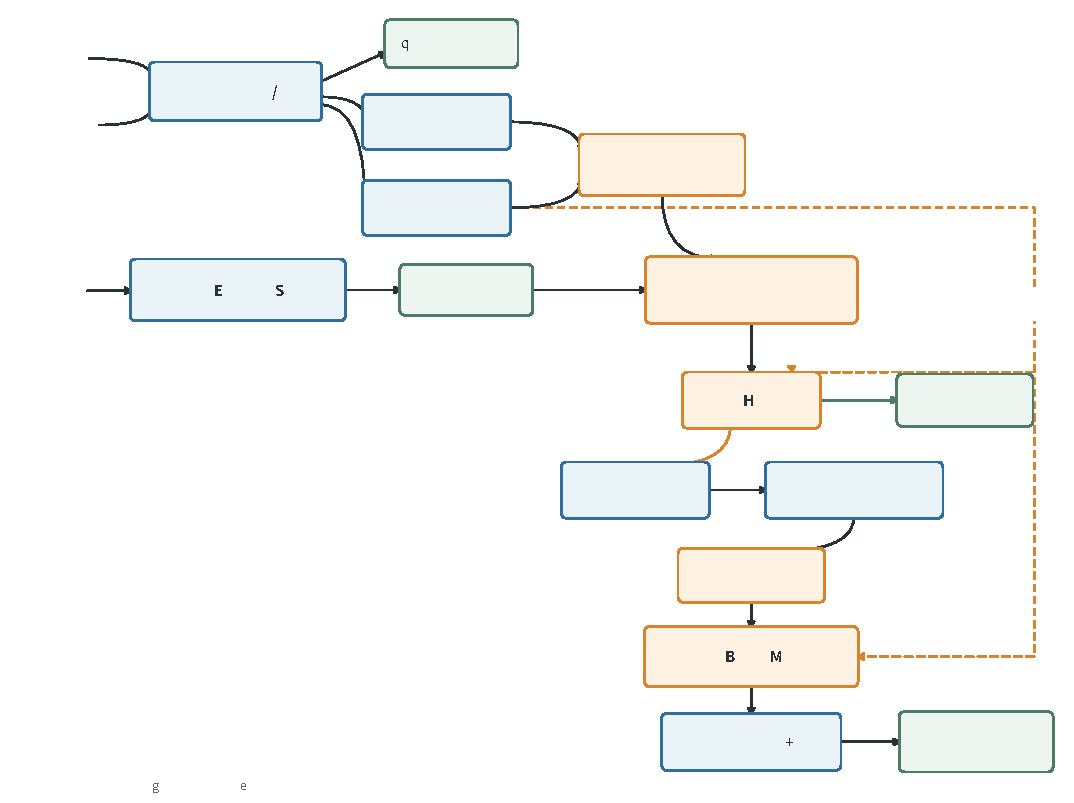
\includegraphics[width=0.96\textwidth]{figures/framework.pdf}%
  }{%
    \missingfigure{总体框架图待绘图任务生成：\texttt{figures/framework.pdf}}%
  }
  \caption{基于正常模板与多模态验证器的 PCB 缺陷检测结果复核总体框架。基础检测器与模板差异模块产生双来源候选。复检门选择调用对象，接受门和安全规则约束修改动作。类别感知融合输出检测结果与审计日志。}
  \label{fig:framework}
\end{figure*}

统一候选先经过复检门。低风险 DET 或 BOTH 候选沿用检测器结果，低风险 DIFF 候选默认拒绝。高风险且位于调用预算内的候选才构造 A2 三面板证据卡。三个面板分别是当前候选紧裁剪、正常模板同位置紧裁剪和带候选框的更大上下文。外观差异图与拓扑差异图不进入证据卡。外观与结构分析用于提出 $C_{\mathrm{diff}}$，八维拓扑向量作为复检门和接受门的候选特征。第~\ref{sec:candidates} 节给出这一输入分工的设计与实证依据。

多模态验证器结合 A2 证据卡与封闭知识 $K$，输出缺陷存在性、预测类别、参考可靠性和固定原因码。系统比较该判断、候选来源与检测器结果，再映射为六种动作之一。修改类动作继续经过接受门、配准质量阈值和安全规则。未获接受的提议动作回退到默认处理。M11 执行动作并消解重复框，输出最终检测集合和审计记录。

\subsection{模块划分与职责}

表~\ref{tab:modules} 列出 M0 至 M11 的输入、输出与职责。模块边界按照可复现的数据流划分，差异候选、证据卡和门控特征各自承担单一功能。

\begin{table*}[t]
  \centering
  \caption{EviGate-PCB 十二个模块的职责划分}
  \label{tab:modules}
  \small
  \setlength{\tabcolsep}{4pt}
  \begin{tabular}{@{}p{0.14\textwidth}p{0.22\textwidth}p{0.22\textwidth}p{0.36\textwidth}@{}}
    \toprule
    模块 & 输入 & 输出 & 职责 \\
    \midrule
    M0 基础检测器 & 待检图像 $I$ & 框、类别、校准置信度组成的 $C_{\mathrm{det}}$ & 快速提供具有类别语义的初始检测候选，不承担模板比较。 \\
    M1 配准与光度归一 & $I$、正常模板 $R$ & 对齐模板、配准质量 $q_{\mathrm{reg}}$ & 统一几何坐标和亮度尺度。量化正常模板对齐是否可靠，为破坏性动作提供降级依据。 \\
    M2 外观差异 & $I$、对齐模板 & 外观差异图 $M_{\mathrm{app}}$ 与区域统计 & 描述材料增减和灰度变化。仅服务于差异候选与门控特征，不作为 A2 证据卡面板。 \\
    M3 结构差异 & 对齐后的图像对 & 结构差异图 $M_{\mathrm{topo}}$、八维拓扑向量 & 计算容差感知的连通性变化。差异图不进入证据卡，拓扑向量作为门控特征。 \\
    M4 差异候选生成 & $M_{\mathrm{app}}$、$M_{\mathrm{topo}}$ 与质量信息 & $C_{\mathrm{diff}}$ & 对差异区域阈值化、过滤和成框，提出可用于恢复漏检的候选假设。 \\
    M5 候选融合 & $C_{\mathrm{det}}$、$C_{\mathrm{diff}}$ & 统一候选 $C$ 与来源标记 & 合并空间一致的候选，标记 DET、DIFF 或 BOTH，并保留动作所需的原框信息。 \\
    M6 复检门 & 检测、差异、拓扑、来源及 $q_{\mathrm{reg}}$ 等候选特征 & 复检风险分数与调用决策 & 在预算内定位更可能被纠正的候选，决定是否调用多模态验证器。 \\
    M7 A2 证据卡 & 高风险候选、$I$、对齐模板 & 三面板视觉证据 & 生成当前紧裁剪、模板紧裁剪和更大上下文，保持对应位置和缩放一致。 \\
    M8 多模态验证器独立判断 & A2 证据卡、封闭缺陷知识 $K$ & 固定 JSON 视觉判断 & 在候选范围内判断缺陷存在性和类别。不自由生成框，不直接执行系统动作。 \\
    M9 动作映射 & 验证器输出、候选来源、检测器结果 & 六类提议动作 & 在模型外比较独立判断与原检测。把结论映射为 keep、remove、relabel、add、reject 或 defer。 \\
    M10 接受门与安全规则 & 候选证据、提议动作、$q_{\mathrm{reg}}$ & 执行或回退决策 & 估计修改是否产生正效用。以动作阈值、配准约束和合法性规则减少有害修正。 \\
    M11 最终融合 & 全部已接受动作与默认结果 & 最终框集合、审计日志 & 执行动作并进行类别感知 NMS，记录候选来源、验证器输出、门控分数及最终决策。 \\
    \bottomrule
  \end{tabular}
\end{table*}

M0 至 M5 确定系统的可复核范围，双来源设计将漏检恢复纳入候选空间。M6 选择调用对象，M7 构造验证输入，M8 输出独立判断。M9 和 M10 决定提议动作是否可以改变结果。第 4 章展开 M1 至 M5，并将 M7 与候选几何一并说明；第 5 章展开 M6、M8、M9 和 M10。M11 的执行规则如下。

\subsection{最终融合与审计（M11）}
\label{subsec:final-fusion}

M11 以基础检测结果为默认集合，只执行通过 M10 的修改类动作。\texttt{remove} 删除对应的检测器原框。\texttt{relabel} 只更新该原框的类别。\texttt{add} 加入 DIFF 候选已有的边界框。\texttt{keep}、\texttt{reject} 和未获接受的提议动作不改变默认集合。\texttt{defer} 在自动评价中同样沿用默认结果，并在审计记录中标为待人工处理。第~\ref{sec:gating} 节的动作合法性、配准质量阈值和回退规则先于本模块执行。

动作执行后，M11 采用 IoU 阈值为 $0.5$ 的类别感知 NMS。同类别重叠框按最终分数降序保留，异类别框不互相抑制。该次序构成同类别冲突的优先级：原有或改类框沿用检测器校准分数，新增框使用接受门概率。删除动作不产生分数，改类动作不改变框坐标。系统不把验证器的文本置信度直接写入检测分数。

每条候选审计记录包含图像与候选标识、来源标记、复检分数与调用状态。记录还包含多模态验证器的结构化输出、提议动作、接受概率和动作执行状态。候选标识可关联 $q_{\mathrm{reg}}$、候选几何和其他门控特征。最终输出另行记录边界框、类别和分数。审计记录据此区分未调用、未接受与已执行三种状态。

\section{双来源候选与外观结构差异证据}
\label{sec:candidates}

基础检测器只能复核已经提出的目标，无法恢复没有检测候选的漏检。正常模板提供同一位置的无缺陷参照，可用于发现检测器未覆盖的变化区域。本章展开 M1 至 M5：先配准正常模板，再计算外观差异和拓扑差异，随后生成并融合候选。M7 依赖候选几何，因此也在本章说明。外观图和拓扑图用于候选生成，但不直接作为多模态验证器的视觉输入。第~\ref{subsec:evidence-card} 节分别报告阶段 C 主消融与阶段 B2 专门对照，说明这一取舍的依据。

\subsection{模板配准与光度归一（M1）}
\label{subsec:registration}

设待检图为 $I$，与其模板编号对应的正常图为 $R$。虽然 DeepPCB 按成对文件提供二者，但文件配对不等于像素级对齐。若直接计算残差，轻微平移和旋转会在铜线边缘形成成片的双边响应，使正常结构被误认为缺陷。M1 因而采用粗到细的两级配准。粗级利用数据目录中的模板标识取得正确参考，并在灰度图像金字塔上估计全局运动；细级以增强相关系数（enhanced correlation coefficient, ECC）为目标优化轻量仿射变换：
\begin{equation}
  \hat{T}=\arg\max_T \operatorname{ECC}\bigl(I,W(R;T)\bigr),
  \qquad R'=W(R;\hat{T}),
  \label{eq:ecc-registration}
\end{equation}
其中 $W(\cdot;T)$ 表示将模板变换到待检图坐标系。仿射模型能够表达数据中的小幅平移、旋转和尺度变化，又比无约束单应模型更不容易把局部缺陷吸收到几何变换中。金字塔上层先处理低频结构和较大位移，下层再修正铜线边缘的亚像素残差。

ECC 未收敛、相关性过低或变换参数越界时，系统回退到 ORB 特征匹配与 RANSAC 单应估计。该分支先在两图中提取二值描述子，以匹配点形成候选对应关系，再用 RANSAC 排除受缺陷和重复线路影响的外点。回退分支的目的不是用更高自由度持续追求较小残差，而是在 ECC 失效时恢复可用的全局对应。若两个分支均不可靠，系统保留基础检测结果，并禁止由模板差异触发自动新增、删除或改类，避免错误参考继续向后传播。

阶段 0 的抽样核查显示，估计平移的绝对值最大为 $8.62$ px，近零变换仅占 $21/50$。DeepPCB 原图近似对齐，但未达到像素级预配准。M1 因而是差异计算前的必要步骤。完整数据实况见第~\ref{sec:experiments} 节。

几何对齐后，本文使用中位数和中位绝对偏差（median absolute deviation, MAD）进行稳健光度归一：
\begin{equation}
  \widetilde I=\frac{I-\operatorname{median}(I)}{\operatorname{MAD}(I)+\epsilon},
  \qquad
  \widetilde R=\frac{R'-\operatorname{median}(R')}{\operatorname{MAD}(R')+\epsilon}.
  \label{eq:mad-normalization}
\end{equation}
中位数削弱整体亮度偏移，MAD 降低少量高亮反射和缺陷像素对尺度估计的影响。阶段 0 统计中，灰度值为 0 或 255 的像素占 $93.99\%$，说明 DeepPCB 接近二值图。本文仍保留光度归一，以处理 JPEG 灰度和待检图特有的强度变化，但不把后续效果归因于连续纹理建模。完整统计见第~\ref{sec:experiments} 节。

M1 同时输出配准质量分 $q_{\mathrm{reg}}\in[0,1]$。ECC 相关系数、ORB/RANSAC 内点率和边缘双向 Chamfer 距离描述几何质量。背景中位差和变换参数越界程度补充残差与参数约束。五类指标组成特征向量 $z^{\mathrm{reg}}$。背景中位差在剔除最高残差区域后计算。系统再用验证样本和合成错位样本校准映射
\begin{equation}
  q_{\mathrm{reg}}=g_{\mathrm{reg}}(z^{\mathrm{reg}}).
  \label{eq:qreg}
\end{equation}
ECC 分支和回退分支由同一质量量纲进入后续模块。$q_{\mathrm{reg}}$ 作为复检门和接受门的输入，也作为配准质量安全开关。低于阈值时，系统停止执行依赖模板的修改并回退到检测器输出。阶段 E 只支持 $q_{\mathrm{reg}}$ 对选定平移强度序列呈下降趋势。在本实验的扰动范围内，配准质量阈值拦截的有害动作数为 0，其保护作用尚未得到实证。完整负面结果见第~\ref{sec:experiments} 节。

\subsection{外观差异与拓扑差异（M2、M3）}
\label{subsec:appearance-topology}

配准和归一后的图像进入两条差异计算路径。外观路径关注材料强度的增减，拓扑路径关注铜线连通关系的改变。二者负责形成差异候选和数值特征，不作为多模态验证器的直接视觉输入。

外观差异由逐像素绝对差和结构相似性残差加权得到：
\begin{align}
  M_{\mathrm{pix}} &= \operatorname{Norm}\bigl(|\widetilde I-\widetilde R|\bigr), \\
  M_{\mathrm{ssim}} &= \frac{1-\operatorname{SSIM}(\widetilde I,\widetilde R)}{2}, \\
  M_{\mathrm{app}} &= \eta_1 M_{\mathrm{pix}}+\eta_2 M_{\mathrm{ssim}}.
  \label{eq:appearance-map}
\end{align}
绝对差对局部铜缺失、额外铜和孔洞变化响应直接，SSIM 残差补充邻域结构与对比度变化。权重 $\eta_1$、$\eta_2$ 只在验证折选择，不在测试折调节。主数据接近二值，$M_{\mathrm{pix}}$ 已包含材料边界信号。SSIM 残差将孤立的强度响应组织为局部结构响应，不用于提取自然图像纹理。

拓扑路径先对当前图和对齐模板执行 Otsu 阈值分割。轻量开闭运算清除孤立噪点和小孔，得到铜区域掩码 $B_I$ 与 $B_R$，再骨架化为 $K_I$ 与 $K_R$。若直接计算 $K_I\mathbin{\mathrm{XOR}}K_R$，不足一个线宽的配准残差也会沿整条线路产生两条平行伪差异。本文在比较前对对方骨架作半径为 $\delta$ 的膨胀，定义容差感知 XOR：
\begin{equation}
  M_{\mathrm{topo}}=
  \bigl(K_I\land\neg\operatorname{Dilate}(K_R,\delta)\bigr)
  \lor
  \bigl(K_R\land\neg\operatorname{Dilate}(K_I,\delta)\bigr).
  \label{eq:tolerant-xor}
\end{equation}
式~\eqref{eq:tolerant-xor} 只保留在对方骨架的 $\delta$ 邻域中无法找到对应点的结构变化。真实断路、桥接和支路增生仍会保留，轻微横向漂移造成的成对边缘响应则被吸收。容差不是单纯的图像平滑，它显式编码“在允许位置误差内视为同一条线路”的匹配关系。

阶段 E 的实测支持容差 XOR 设计。其漏检恢复率为 $23.62\%$，并同时降低正常区域的伪差异。该结果不支持“仅靠扩大异常区域换取召回”的解释。完整对照见第~\ref{sec:experiments} 节。

对每个候选区域，M3 还计算八维局部拓扑向量
\begin{equation}
  t_i=[\Delta n_{cc},\Delta n_{end},\Delta n_{branch},\Delta\chi,
  \Delta L,r_{xor},\Delta A,\Delta P],
  \label{eq:topology-vector}
\end{equation}
其中 $n_{cc}$ 为连通分量数量，$n_{end}$ 为骨架端点数量。$n_{branch}$ 为分叉点数量，$\chi$ 为 Euler 数。$L$ 为骨架长度，$r_{xor}$ 为容差 XOR 占比。$A$ 和 $P$ 为铜区域面积与轮廓周长。各差值均在当前区域和模板同坐标区域之间计算。该向量不充当六类缺陷的硬规则分类器，而以连续特征描述结构变化。阶段 B2 否定了把拓扑图直接放入证据卡的做法，但没有检验该向量作为门控特征的独立增量。

\subsection{差异候选生成（M4）}
\label{subsec:diff-candidates}

M4 将连续差异图转换为有限数量的候选。阈值估计的关键是限定正常区域，而不是对含缺陷的整图直接取高分位数。设训练折或验证折中的非缺陷像素集合为 $\Omega_N$，外观阈值定义为
\begin{equation}
  \tau_{\mathrm{app}}=Q_{1-\alpha}
  \left(M_{\mathrm{app}}(x)\mid x\in\Omega_N\right),
  \label{eq:normal-quantile}
\end{equation}
并以相同原则确定拓扑差异阈值。整图分位数会把缺陷像素纳入“正常残差”经验分布。缺陷面积或残差增大时，高分位阈值也会升高，真实响应可能落到阈值以下。早期故障诊断表明，整图分位数会抬高阈值。改用正常区域估计后，前序配置在 IoU 为 0.3 时的漏检恢复候选率为 $0.318$。该结果支持按正常区域估计阈值，完整诊断见第~\ref{sec:experiments} 节。

外观和拓扑二值响应采用逻辑或合并：
\begin{equation}
  M_{\mathrm{bin}}=
  \mathbf{1}[M_{\mathrm{app}}>\tau_{\mathrm{app}}]
  \lor
  \mathbf{1}[M_{\mathrm{topo}}>\tau_{\mathrm{topo}}].
  \label{eq:candidate-mask}
\end{equation}
随后执行开运算、闭运算和孔洞填充，再提取连通域。面积上下界和形状约束作用于连通域掩码，外接框只用于匹配与裁剪。连通域面积指差异响应像素数，外接框面积指包围这些像素的矩形面积。DeepPCB 的最小面积标注框为 $20\times20$ px，后者为 $400$ px$^2$。若把连通域面积下界也设为 400，稀疏响应会过滤掉小缺陷。阶段 A 因而将该下界降至 150；对应的 IoU 0.3 召回极差贡献为 $0.328$。完整调参结果见第~\ref{sec:experiments} 节。

阶段 A 在检测器未参与训练的 val 折完成参数扫描，避免检测器训练样本进入漏检分母。推荐配置的 IoU 0.3 漏检恢复候选率为 $0.625$。实测支持差异路径用于提出漏检候选，也显示后续仍需由复检门控制调用成本。完整扫描见第~\ref{sec:experiments} 节。

参数扫描以搜索范围内的 IoU 0.3 召回极差衡量敏感性。阈值估计的影响最大，极差为 $0.524$；面积下界次之。该排序与整图分位数抬高阈值、连通域面积不同于外接框面积两项分析一致。完整因素排序见第~\ref{sec:experiments} 节。

每个差异候选保留三组扩展属性。外观属性包括残差均值、最大值、高分位数和超阈值面积占比。拓扑属性包括 XOR 面积和式~\eqref{eq:topology-vector} 的局部向量。融合与质量属性包括检测框重叠关系和 $q_{\mathrm{reg}}$。这些属性用于候选融合，也作为第 5 章复检门的输入。它们扩展了式~\eqref{eq:cdiff} 的最小记录结构。

\subsection{候选融合（M5）}
\label{subsec:candidate-fusion}

设基础检测器候选为 $C_{\mathrm{det}}$，差异候选为 $C_{\mathrm{diff}}$。M5 在二者之间构图。一对框的 IoU 不小于 $0.3$ 时连接对应节点；一个框的中心落入另一个按局部尺度扩张后的框时也建立连接。连通节点聚为统一候选，并标记为 \texttt{DET}、\texttt{DIFF} 或 \texttt{BOTH}。IoU 阈值与漏检候选召回的评价口径一致。中心点规则用于处理位置一致但重叠较小的细长差异连通域。

融合记录同时保留检测器原框、差异外接框和融合上下文框。多模态验证器查看覆盖两种来源的融合区域。\texttt{keep}、\texttt{relabel} 和 \texttt{remove} 始终作用于检测器原框，避免上下文扩张改变定位。\texttt{BOTH} 已包含检测器框，因此不允许执行 \texttt{add}。若检测框与差异框的 IoU 小于 $0.1$，系统将其拆回两个独立候选。二者随后分别进入 \texttt{DET} 与 \texttt{DIFF} 流程。该规则防止空间一致性不足的候选获得双来源标记。（融合阈值与动作约束来源：开发规格书第 3.6 节。）

三类来源承担不同职责。\texttt{DET} 保留检测器类别和校准置信度，覆盖正确检测、误报和错分类。\texttt{DIFF} 不携带检测类别，用于提出潜在漏检位置。\texttt{BOTH} 表示检测语义与模板变化在空间上相互支持。融合只建立候选级对应关系，不决定最终动作。

\subsection{证据卡（M7）}
\label{subsec:evidence-card}

M7 采用 A2 三面板证据卡，不采用被否定的 A6 六面板配置。P1 是当前待检图的候选紧裁剪。P2 是配准后正常模板在相同坐标和尺度下的紧裁剪。P3 是带候选位置标记的更大上下文。P1 与 P2 支持当前位置的直接比较，P3 保留线路走向和相邻焊盘关系。三个面板保持固定次序、坐标对应和显示范围。

证据分辨率由缺陷尺度决定。阶段 0 统计给出的框宽和框高中位数分别为 35 px 与 33 px。P1 和 P2 使用相同插值方式与几何尺度，上采样到 $256\times256$。P3 使用更大的原图上下文，并标记候选位置。上采样只改善显示尺度，不创造新结构。完整尺度统计见第~\ref{sec:experiments} 节。

外观差异图和拓扑差异图最终不进入证据卡。阶段 C 的 200 候选主消融中，A4 的存在性 F1 为 $0.7571$，略高于 A2 的 $0.7553$。该差异落在置信区间内，未证明拓扑图相对 A2 带来增量。阶段 C 的其余附加差异证据同样没有证明稳定增量。完整主消融见第~\ref{sec:experiments} 节。

阶段 B2 采用不同的专门对照设置。该实验固定候选、提示词骨架和解码设置，共进行 450 次对照。A2 为 $0.8082$，高于全部包含外观图、拓扑图或数值拓扑摘要的变体。该结果支持从最终证据卡中移除显式差异视觉输入。阶段 C 回答主消融中的增量是否成立，阶段 B2 检查专门构造的差异证据变体。两组数值不合并比较。

阶段 B2 还检查了渲染尺度和候选来源两项混淆因素。$M_{\mathrm{app}}$ 固定截断到 $[0,1]$ 并使用固定色标，拓扑图采用固定三色映射，因此不存在逐图自动拉伸。按 \texttt{DET}、\texttt{DIFF} 和 \texttt{BOTH} 分别统计时，加入外观差异图的 A3 均低于 A2。固定渲染排除了显示尺度漂移，分来源比较削弱了配准残差污染这一解释。现有结果只支持“显式差异视觉输入未带来稳定增量”，不对注意力分散等机制原因作推断。

这项负面结论不否定 M2 和 M3 的候选生成作用。阶段 A 的候选召回实测支持漏检候选生成。阶段 E 的容差 XOR 实测支持结构伪差异抑制，详见第~\ref{sec:experiments} 节。本文据此重新划分信息流。A2 三面板证据卡是多模态验证器的视觉输入。外观残差统计、八维拓扑向量和 $q_{\mathrm{reg}}$ 是复检门与接受门的结构化特征。第 5 章说明门控中的具体使用方式。

\section{分级复核与保守修正}
\label{sec:gating}

候选级复核同时受到调用成本与修改风险的约束。对全部候选调用多模态大模型会使计算开销随候选数线性增长。若直接用模型结论覆盖检测结果，错误判断还会抵消基础检测器的性能。本文用四个模块分离调用选择、候选验证、动作映射和动作执行权限。复核调用选择门 M6 简称复检门，只决定哪些候选进入多模态验证器。多模态验证器 M8 给出独立视觉结论，M9 将结论映射为提议动作，接受门 M10 判断是否执行。复检门优化有限预算下的错误覆盖，接受门约束修改风险，二者不能由同一阈值替代。

\subsection{复检门（M6）}
\label{subsec:review-gate}

设候选 $x_i$ 的基础检测结果及外部证据特征为 $z_i^{\mathrm{review}}$。复检门不判断候选处是否存在缺陷。其监督目标是预测该候选是否包含可由多模态验证器处理且有可执行修正动作的错误：
\begin{equation}
 y_i^{\mathrm{review}}=
 \mathbb{I}\!\left[x_i\text{ 对应可修复的误报、漏检或错分类}\right].
 \label{eq:review-label}
\end{equation}
该定义区分“困难样本”和“可修复错误”。低置信度的正确检测不应占用有限调用预算。高置信度误报和差异分支发现的漏检候选则是正例的主要来源。复检门输出风险分数 $r_i=g_r(z_i^{\mathrm{review}})$，并在调用率预算 $b$ 下选择分数最高的前 $b$ 比例候选。阈值随预算变化。复检门不读取多模态验证器输出，也不决定检测框的增删改。

输入特征覆盖检测器不确定性、候选来源、参考差异和几何属性。检测器侧使用温度校准后的置信度、类别 margin 与预测熵。来源标记采用 DET、DIFF、BOTH 的独热表示，并保留检测框与差异框的重叠信息。外观证据包括残差均值、95 分位数和超过差异阈值的面积比例。8 维拓扑向量描述连通分量、端点、分支点、欧拉数、骨架长度、拓扑异或面积、区域面积和周长的变化。配准质量 $q_{\mathrm{reg}}$ 表示正常模板证据的可信程度。框宽、框高和长宽比补充尺度信息。特征向量为
\begin{equation}
 z_i^{\mathrm{review}}=[p_i^{cal},m_i,H_i,s_i,u_i^{\mathrm{app}},t_i,q_{\mathrm{reg}},w_i,h_i,w_i/h_i],
 \label{eq:review-features}
\end{equation}
其中 $s_i$ 表示来源及来源间重叠特征，$u_i^{\mathrm{app}}$ 表示外观残差统计，$t_i\in\mathbb{R}^{8}$ 表示拓扑向量。拓扑差异图在证据消融后不再作为多模态验证器的视觉输入，其数值向量仍作为复检门的结构化特征。

本文比较 L2 正则 Logistic 回归与 LightGBM。Logistic 便于解释特征方向，LightGBM 可描述特征间的非线性交互。阶段 C 的五折 OOF 数据包含 51222 个候选，正例率约为 2.1\%。表~\ref{tab:review-gate-models} 给出设计阶段的跨折结果。LightGBM 的 PR AP 为 0.4311，Logistic 为 0.1839，前者约为后者的 2.3 倍。两者的 ROC AUC 分别为 0.9227 和 0.7909。负例占多数时，PR AP 更直接反映少数正例的排序质量。方法上两类模型均可用于复检门。阶段 D 按预注册协议固定使用 Logistic 主模型，LightGBM 仅作对照。本文未依据测试结果更换主模型。完整比较见第~\ref{sec:experiments}章。

\begin{table}[t]
  \centering
  \caption{阶段 C 复检门的五折 OOF 性能}
  \label{tab:review-gate-models}
  \begin{tabular}{lcc}
    \hline
    模型 & PR AP & ROC AUC \\
    \hline
    Logistic & 0.1839 & 0.7909 \\
    LightGBM & \textbf{0.4311} & \textbf{0.9227} \\
    \hline
  \end{tabular}
\end{table}

\subsection{多模态验证器（M8）与动作映射（M9）}
\label{subsec:mllm-action-map}

多模态验证器采用去锚定输入原则。模型查看当前候选紧裁剪、局部上下文和对齐后的正常模板紧裁剪，不读取检测器类别、置信度和系统期望动作。模型先作出视觉判断，系统再将其与检测结果比较。多模态验证器不能在整幅图像中搜索缺陷，只能验证 DET、DIFF 或 BOTH 分支给出的候选区域。该任务属于封闭候选验证。

缺陷类别限于数据集定义的六类。标签为 open、short、mousebite、spur、pinhole 和 spurious\_copper。存在性只能取 true、false 或 null。类别字段在六类之外只允许 normal 与 uncertain。参考可靠性、外观模式、拓扑模式、证据强度和原因码均使用固定枚举。冻结的 JSON Schema 设有 defect\_present 和 predicted\_class 字段。reference\_reliability 记录参考可靠性。appearance\_pattern 与 topology\_pattern 记录两类模式。evidence\_strength 与 reason\_codes 分别记录证据强度和原因码。自由文本对照的 JSON 可解析率为 0.0000，无法稳定支持动作映射、接受特征构造和审计记录。因此主实验采用结构化输出，解析失败或字段越界均标记为无效。系统不从自然语言中猜测动作，完整实验结果见第~\ref{sec:experiments}章。

M9 在多模态验证器外部执行确定性映射，规则见表~\ref{tab:action-map}。DET 和 BOTH 候选包含基础检测框。独立结论为 normal 时提议 remove；结论为缺陷且类别与检测器一致时 keep。只有新类别非 uncertain、拓扑证据支持新类别并反驳原类别时，系统才提议 relabel。无法形成确定结论时 defer。DIFF 候选不依附已有检测框。受支持的缺陷结论映射为 add，normal 映射为 reject，不确定结论映射为 reject 或 defer。BOTH 候选不能通过 add 生成重叠框。多模态验证器只描述视觉结论，系统侧映射保留最终修改权限。

\begin{table}[t]
  \centering
  \caption{候选来源与独立结论的动作映射}
  \label{tab:action-map}
  \begin{tabular}{lll}
    \hline
    来源 & 独立结论 & 提议动作 \\
    \hline
    DET/BOTH & normal & remove \\
    DET/BOTH & 缺陷且类别相同 & keep \\
    DET/BOTH & 缺陷且类别不同、证据一致 & relabel \\
    DET/BOTH & uncertain & defer/keep \\
    DIFF & 缺陷 & add \\
    DIFF & normal & reject \\
    DIFF & uncertain & reject/defer \\
    \hline
  \end{tabular}
\end{table}

动作优先级由五折基础检测错误分解决定。可纠错空间包含漏检 947 个、误报 636 个和错分类 61 个。三者分别占 57.6\%、38.7\% 和 3.7\%。prompt 先判断候选处是否存在受支持缺陷。该判断服务于 DIFF 候选的 add 动作和 DET/BOTH 候选的 remove 动作。relabel 的理论收益上限最小，错误判断还会把位置正确的检测转化为错分类。因此，relabel 同时要求封闭类别、非 uncertain 结论和类别拓扑一致性。该设计按错误构成分配三类动作的判断能力和风险额度，完整错误分解见第~\ref{sec:experiments}章。

prompt 版本实验显示存在性 F1 与 remove 可用性之间存在权衡。v1 的缺陷存在性 F1 为 0.7678，高于 v2 的 0.7347。v1 的 normal 判定率为 0.31，低于 v2 的 0.39。提高 normal 判定率有助于识别误报，但会降低整体存在性 F1。remove 依赖 normal 结论，因为 DET/BOTH 候选只有在模型否定缺陷时才会提出删除。早期开发 smoke 实验中，v1 的 normal 判定率为 0.000，remove 因而不可用。v2 加强 normal 引导并接受存在性 F1 下降，目标是恢复双向纠错能力，而不是证明 v2 全面优于 v1。第~\ref{sec:experiments}章同时报告两个指标，以呈现动作分布的变化。

\subsection{接受门（M10）与安全规则}
\label{subsec:acceptance-gate}

复检门放行只表示候选值得查看，多模态验证器给出提议动作也不表示该动作安全。接受门预测执行每个提议动作是否产生正效用。给定当前预测集合 $\hat{Y}$、真值 $Y^{*}$ 和动作 $a_i$，训练标签定义为
\begin{equation}
 y_i^{\mathrm{accept}}=
 \mathbb{I}\!\left[U(\hat{Y}\oplus a_i,Y^{*})>U(\hat{Y},Y^{*})\right],
 \label{eq:accept-label}
\end{equation}
其中 $\oplus$ 表示执行动作。删除原始误报构成 remove 的正效用标签。将已匹配位置改为正确类别构成 relabel 的正效用标签。添加匹配原漏检真值的差异框构成 add 的正效用标签。损害检测结果或没有改善的修改均为负例。

不同动作的样本机制、风险和正例率不同。因此，接受门按 remove、relabel、add 分开训练，不将动作独热编码后混合拟合。输入先沿用复检特征，再加入多模态验证器的存在性与类别结论。其他输入包括证据强度、参考可靠性、外观一致性、拓扑一致性和 JSON 有效标记。最终执行条件为
\begin{equation}
 \operatorname{Apply}(a_i)=
 \mathbb{I}[g_{a_i}(z_i^{\mathrm{accept}})\geq \tau_{a_i}]
 \land \operatorname{SafetyRule}(a_i),
 \label{eq:accept-rule}
\end{equation}
其中 $g_{a_i}$ 是动作专属接受模型，$\tau_{a_i}$ 是动作阈值。模型概率只提供统计证据，不能绕过硬安全规则。

阶段 C 的五折训练分布支持按动作建模。remove 每折约 800 个样本，正例为 26 到 46 个。add 每折约 12000 个样本，正例为 39 到 55 个。两类数据均高度不平衡，但仍包含正负例。relabel 每折约 2300 个样本，正例仅为 0 到 5 个，fold3 为 0。全数据只有 61 个错分类。折隔离和提议动作筛选后，这些数据无法支持稳定的 relabel 接受模型。类别权重或过采样不能消除这一限制。fold3 的标签单一，因而触发保守退化；relabel 模型不输出接受概率，系统拒绝该动作。其他折即使能够拟合，也必须服从更高阈值和拓扑一致性检查。完整分布见第~\ref{sec:experiments}章。

硬安全规则按动作后果设置。remove 会丢弃已有检测，因而使用三类动作中的最高阈值，且只作用于 DET 或 BOTH 候选。relabel 只能在封闭的六类标签内执行。多模态验证器的类别结论必须与拓扑模式一致，来源也必须包含原检测框。add 只能采用已有 DIFF 候选的确定性边界，不允许多模态验证器生成坐标。BOTH 候选已有检测框，不能执行 add。配准质量 $q_{\mathrm{reg}}$ 低于阈值时，系统禁止 remove、relabel 和 add。在选定平移序列中，$q_{\mathrm{reg}}$ 随扰动增强而总体下降，可用作可靠性指标。但阈值 0.5 拦截的有害动作数为 0。当前实验尚未证实该安全规则的保护作用，详见第~\ref{sec:experiments}章。JSON 解析失败、字段非法或动作冲突时，系统保留基础检测器输出或将候选交由人工处理。

训练不足时，兜底方向决定最坏情况风险。若样本少于最低要求或训练标签单一，接受概率固定回退为 0，并拒绝全部修改。早期实现采用接受式退化，多模态验证器的错误会直接进入最终结果。保守退化则返回未修改基线，并放弃当前数据无法支持的收益。该规则对 relabel 尤其关键，因为 fold3 没有正例。

\subsection{防泄漏与门控训练协议}
\label{subsec:gating-protocol}

数据按 PCB 模板组执行五折 GroupKFold，同一模板的旋转图和衍生图不能跨越训练与测试边界。第 $i$ 折以该折图像为 test，以第 $(i+1)\bmod 5$ 折为 val，其余三折训练检测器。五折本身已经覆盖全部 1500 张图，每张图恰好在一折中作为 test，且产生该图预测的检测器从未见过该图。将五个 test 折的输出拼接即可得到完整 OOF 候选集合，不需要再在每个外层折中嵌套检测器交叉拟合。

若在每个外折内重新构造四折检测器预测，两层折叠需要 20 次训练。本文协议只训练 5 次检测器，同时使每条门控记录来自样本外预测。先用全数据训练检测器再构造门控标签会泄漏检测分数和错误分布。温度校准、工作点选择和 prompt 定稿均使用对应 val 折，不接触当前 test 折。

门控层再执行一次按折隔离。评价第 $i$ 折时，复检门与三个动作接受门只能使用其他四折的 OOF 候选及其标签训练。当前第 $i$ 折只用于排序、调用和最终评价。形式化地，门控训练集为 $\mathcal{D}_{g}^{(-i)}=\bigcup_{j\neq i}\mathcal{D}_{\mathrm{OOF}}^{(j)}$，评价集为 $\mathcal{D}_{\mathrm{OOF}}^{(i)}$。候选特征、正效用标签和阈值选择均遵守这一边界。最终报告汇总五个互斥评价折，避免检测器预测泄漏与门控标签泄漏叠加。

接受门的提议动作训练样本由冻结的确定性证据代理生成，以节省多模态验证器调用。该选择保持折间隔离，但会造成代理动作与真实动作之间的训练分布偏移。因此，当前接受概率不能解释为对任意多模态验证器输出均已校准。部署时应记录真实提议，并在样本充足后按相同折隔离原则重训动作模型。样本不足期间继续采用拒绝式保守退化。

\subsection{分级复核的成本收益}
\label{subsec:gating-cost-benefit}

RQ3 在 5\%、10\%、20\%、40\%、60\% 和 100\% 六个调用预算上比较候选选择与动作接受策略。复检门的评价依据是相同调用率下的可修复错误覆盖，而不是被调用候选的平均置信度。5\% 预算下，预注册的 Logistic 复检门取得 0.4649 的错误候选复核召回，随机选择为 0.0315。两者调用数相同，前者找到的可修复错误为后者的 14.8 倍。本文用有害修正率（Harmful Correction Rate, HCR）度量动作风险。该指标从随机策略的 0.9633 降至 0.6813。结果支持用结构化特征排序候选，但 0.6813 的 HCR 也表明复检门不能替代动作级保护。图~\ref{fig:hcr-call-rate} 展示 HCR 随调用预算的变化，完整实验设置见第~\ref{sec:experiments}章。

\begin{figure}[t]
  \centering
  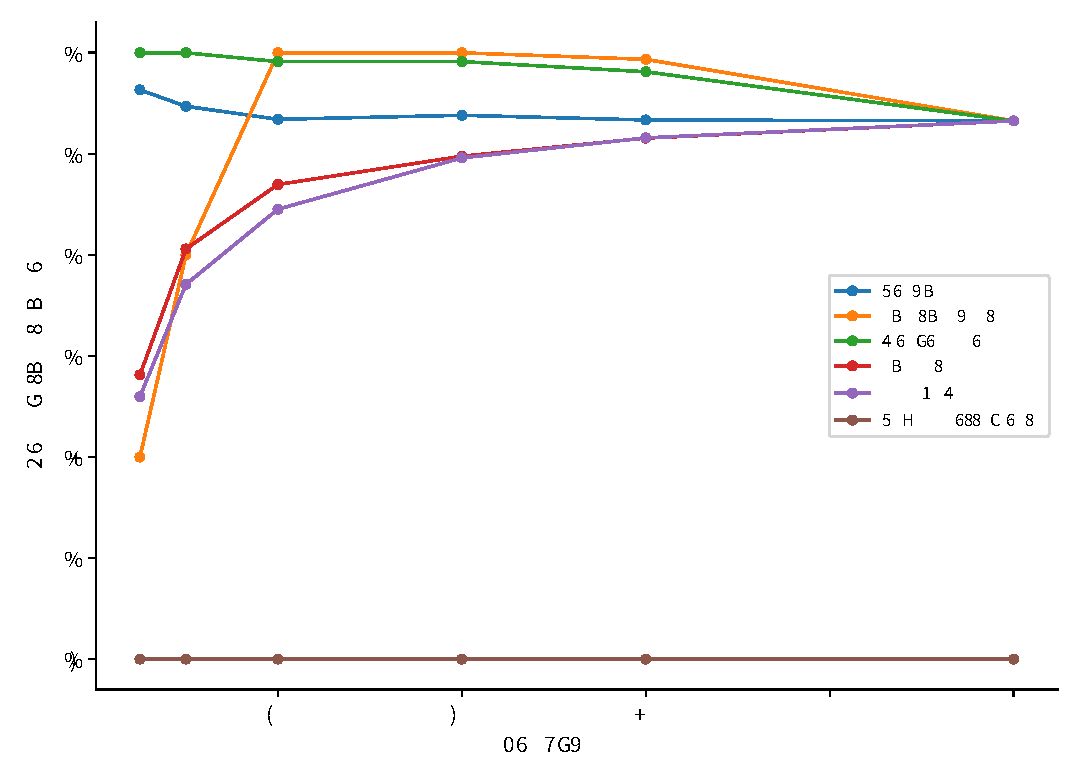
\includegraphics[width=\columnwidth]{figures/hcr_call_rate.pdf}
  \caption{不同调用预算下的有害修正率。学习式复检排序在低预算区间优于随机选择，接受门进一步减少高风险动作。}
  \label{fig:hcr-call-rate}
\end{figure}

提议动作未经接受门筛选时，最终 F1 随预算下降。5\% 和 20\% 预算下的 F1 分别为 0.9088 和 0.9015。60\% 和 100\% 预算下则为 0.8820 和 0.8660。调用增加会累积错误动作。加入接受门后，5\% 和 20\% 预算下的 F1 分别为 0.9117 和 0.9115。60\% 和 100\% 预算下均为 0.9115。表~\ref{tab:acceptance-budget} 汇总这四个预算点。基础工作点 B1 为 0.9118。有接受门的 0.9115 至 0.9117 与基线无统计差异，不能解释为数值不低于基线。图~\ref{fig:f1-call-rate} 显示，无接受门曲线随预算下降，双门控曲线保持在基线水平。

\begin{figure}[t]
  \centering
  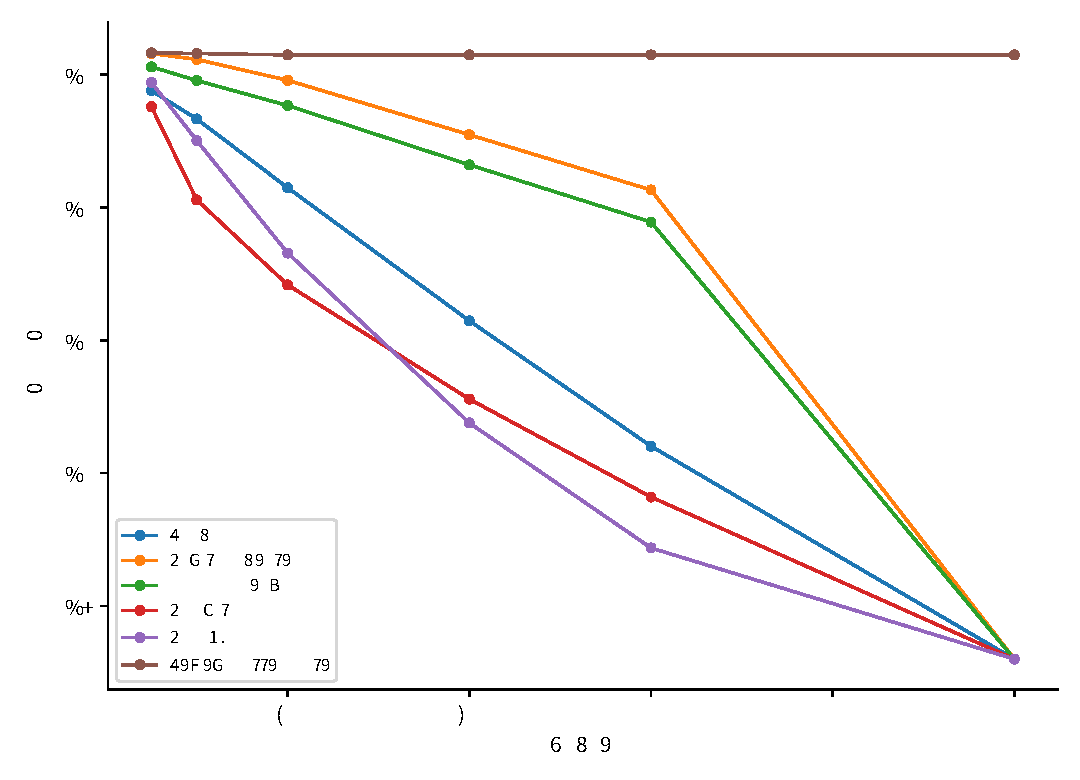
\includegraphics[width=\columnwidth]{figures/f1_call_rate.pdf}
  \caption{调用预算与最终 F1 的关系。缺少接受门时，增加调用会累积错误动作；采用接受门后，各预算点保持稳定。}
  \label{fig:f1-call-rate}
\end{figure}

\begin{table}[t]
  \centering
  \caption{接受门对预算曲线的影响}
  \label{tab:acceptance-budget}
  \begin{tabular}{ccc}
    \hline
    调用预算 & 无接受门 F1 & 有接受门 F1 \\
    \hline
    5\%   & 0.9088 & 0.9117 \\
    20\%  & 0.9015 & 0.9115 \\
    60\%  & 0.8820 & 0.9115 \\
    100\% & 0.8660 & 0.9115 \\
    \hline
  \end{tabular}
\end{table}

安全规则不消除推理成本。多模态验证器的单候选平均时延为 29.1 秒，P95 为 41.4 秒。调用预算从 5\% 增至 100\% 时，平均每图 token 消耗从 123 增至 2519，接近线性增长。100\% 调用对应最高成本，也在无接受门时产生最低 F1。复检门压缩调用量，接受门减少调用后的错误修改，二者分别作用于成本与风险。

端到端结果界定了双门控的作用范围。接受门将无门控方案的 HCR 从 0.9326 降至 0.4000，并把正确检测误删控制在 2 次。它没有完全阻断有害修正。有接受门的预算曲线保持在基线水平，但未证明检测精度提高。当前净收益仍受多模态验证器判断质量限制。系统因此把有限调用优先分配给高风险候选，并在训练证据不足时拒绝修改。

\section{实验设计、结果与分析}
\label{sec:experiments}

本章回答四个研究问题。RQ1考察视觉证据对多模态验证器候选级判断能力的影响。RQ2检验复核系统能否在完整检测流程中纠正误报、漏检和错分类。RQ3分析复检门与接受门在不同调用预算下的效率和可靠性。RQ4考察配准扰动、差异表示和检测器替换对系统行为的影响。除专门说明的候选级诊断实验外，主结果均来自按模板组隔离的五折测试。正面发现、统计上不显著的结果和性能退化均纳入报告，整体结论不以单个折或单个预算点代替。

\subsection{实验设置}
\label{subsec:exp_setup}

\subsubsection{数据集及严格划分}

实验采用DeepPCB数据集\cite{tang2019deeppcb}。按仓库中的实际列表文件和图像文件核查，数据集包含1500对待检图与正常模板。官方\texttt{trainval}包含1000对，官方\texttt{test}包含500对。全部图像均为$640\times640$像素的JPEG图像，主体为单通道灰度图。1500个标注文件共包含10013个缺陷框。缺陷框分为open、short、mousebite、spur、spurious copper和pin-hole六类。每幅图的缺陷框数中位数为7。缺陷框宽度和高度的中位数分别为35和33像素。候选级复核处理的是局部细粒度目标，而非整图级异常。

官方划分不能直接支撑本文的主结论。数据目录可以稳定还原11个模板组，其中7个模板组同时出现在官方\texttt{trainval}和\texttt{test}中。同一模板组的板图会分别进入训练集和测试集，检测器因而接触到二者共享的板级结构。这种组间泄漏会低估跨模板泛化难度，并抬高检测和复核结果。本文仅用官方划分对照既有结果，不据此判断方法有效性。

主实验采用\texttt{GroupKFold}五折划分，以模板组作为不可拆分的分组单元。第$i$折的测试组在该折的训练和验证数据中完全不可见，验证集取下一折，其余三折用于训练检测器。评价第$i$折的门控模型时，只使用其余折产生的折外候选训练，防止门控阶段重新引入样本泄漏。11个模板组的规模从14对到325对不等，最大组与最小组相差23.21倍，因此各折样本量不能强行等分。表~\ref{tab:fold_composition}列出了实际测试组成，五折共覆盖1500对图像，每个图像对恰好作为测试样本一次。

\begin{table*}[t]
  \centering
  \caption{按模板组隔离的五折测试集组成}
  \label{tab:fold_composition}
  \setlength{\tabcolsep}{5pt}
  \begin{tabular}{clrr}
    \hline
    折 & 测试模板组 & 图像对数 & 占全部数据比例 \\
    \hline
    fold\_0 & group20085 & 325 & 21.67\% \\
    fold\_1 & group00041、group50600 & 300 & 20.00\% \\
    fold\_2 & group12300、group13000 & 314 & 20.93\% \\
    fold\_3 & group12000、group12100、group44000 & 260 & 17.33\% \\
    fold\_4 & group77000、group90100、group92000 & 301 & 20.07\% \\
    \hline
    合计 & 11个模板组 & 1500 & 100.00\% \\
    \hline
  \end{tabular}
\end{table*}

\subsubsection{基础检测器与多模态验证器}

基础检测器采用YOLOv8s。每折在三个训练折上训练，在独立验证折上选择F1最优工作点，并在测试折上输出折外预测。低置信度阈值0.001只用于计算mAP，不用于报告部署工作点的Precision、Recall和F1。五折检测器的mAP@0.5为$0.9580\pm0.0164$，mAP@0.5:0.95为$0.7135\pm0.0407$。验证集选定工作点上的Precision为$0.9264\pm0.0291$。Recall为$0.8964\pm0.0469$，F1为$0.9105\pm0.0312$。折间F1从0.8721到0.9522，反映了模板隔离后不同板型的难度差异。因此，结果同时报告均值和标准差。

多模态验证器只接收已经定位并放大的证据卡，不在整幅图上自由生成检测框。主后端为本机Codex CLI，模型为\texttt{gpt-5.6-sol}。推理强度设为low，并采用确定性解码。输入由当前紧裁剪、正常模板和上下文组成。JSON Schema将输出约束为固定字段；解析失败时，系统保持基础检测结果。默认协议隐藏检测器类别和置信度。验证器独立判断缺陷是否存在及其类别，系统再将判断映射为keep、remove、relabel或add。keep、remove和relabel始终作用于检测器原框。add只能接受已有差异候选，验证器没有任意造框权限。所有响应按候选、证据配置、模型和解码参数缓存，累计真实调用约7000次。12路并发下实测吞吐上限约26次每分钟，单候选平均墙钟时间约29秒。该成本要求系统选择性调用验证器。

\subsubsection{评价指标与统计方法}

常规检测指标包括Precision、Recall、F1、mAP@0.5、mAP@0.5:0.95和各类别AP。本文另定义五个指标衡量复核动作。设基础检测器的误报、漏检、错分类和正确检测数量分别为$N_{\mathrm{FP}}^0$、$N_{\mathrm{FN}}^0$、$N_{\mathrm{MC}}^0$和$N_{\mathrm{TP}}^0$。误报修正率FPCR是正确删除的原始误报数与$N_{\mathrm{FP}}^0$之比。漏检恢复率MDRR是新增匹配的原始漏检数与$N_{\mathrm{FN}}^0$之比。类别修正准确率MCCA是正确重分类数与$N_{\mathrm{MC}}^0$之比。正确检测保留率TPRR是复核后仍正确的原始TP数与$N_{\mathrm{TP}}^0$之比。有害修正率HCR是降低检测效用的已接受修改数与全部已接受修改数之比。TPRR衡量系统是否破坏原本正确的检测，HCR衡量已执行修改的风险。

成本指标包括验证器调用率、每图调用次数、单候选平均时延和P95时延、每图输入token数以及配准失败回退率。RQ1在同一批候选上比较不同证据配置。置信区间采用按图像聚类的bootstrap，避免把同一图像中的多个候选视为独立样本。RQ2对Full与基础工作点进行2000次按图像聚类的配对bootstrap。端到端指标报告五折均值与折间标准差。所有门控阈值均由验证折选择，并在测试前冻结。

\subsection{可纠错空间分析}
\label{subsec:correctable_space}

在评价复核方法之前，需要先确定基础检测器留下了哪些错误。本文按IoU匹配和类别一致性将工作点输出分解为正确检测、错分类、误报、漏检和纯定位错误。纯定位错误表示检测器已经对目标作出响应，但定位未达到正式匹配阈值。这类错误与三类可通过删除、新增或重分类动作直接处理的错误分开统计。表~\ref{tab:error_decomposition}给出五折结果。

\begin{table*}[t]
  \centering
  \caption{五折基础检测器错误分解}
  \label{tab:error_decomposition}
  \setlength{\tabcolsep}{7pt}
  \begin{tabular}{crrrrrr}
    \hline
    折 & TP & 错分类 & 误报 & 漏检 & 纯定位错误 & 可纠错空间 \\
    \hline
    fold\_0 & 2085 & 6  & 216 & 335 & 2  & 557 \\
    fold\_1 & 1987 & 9  & 166 & 77  & 1  & 252 \\
    fold\_2 & 1894 & 8  & 24  & 148 & 1  & 180 \\
    fold\_3 & 1608 & 23 & 134 & 118 & 10 & 275 \\
    fold\_4 & 1408 & 15 & 96  & 269 & 9  & 380 \\
    \hline
    合计 & 8982 & 61 & 636 & 947 & 23 & 1644 \\
    \hline
  \end{tabular}
\end{table*}

可纠错空间是错分类、误报和漏检之和，共1644项。漏检947项，占57.6\%，是最大错误来源。误报636项，占38.7\%；错分类61项，占3.7\%。只复核检测器已经提出的框，最多能处理误报和错分类，无法触及超过一半的潜在纠错空间。差异候选用于提出检测器未覆盖的位置，再由验证器决定是否新增。错分类的基数只有3.7\%，限制了重分类动作对总体F1的最高贡献。

折间分布同样不均衡。fold\_0有335个漏检和216个误报，可纠错空间为557。fold\_2只有180项可纠错错误，其中误报仅24个。单折结果会偏置复核收益和风险估计。五折隔离既防止模板泄漏，也覆盖不同的误报与漏检构成。RQ2的Oracle分析使用完整固定候选集计算候选覆盖上界，并区分“没有提出候选”与“候选已提出但验证器判断错误”。

\subsection{RQ1：证据消融}
\label{subsec:rq1}

RQ1固定候选、模型、提示词骨架和解码参数，只改变证据卡内容。A0仅给出当前紧裁剪，A1加入上下文，A2再加入配对正常模板。A3和A4分别加入外观差异与拓扑差异，A5和A6组合更多证据。七组主消融及四组附加对照均在相同的200个候选上评价。候选级任务判断候选位置是否存在真实缺陷。F1相对A0的差值采用按图像聚类的bootstrap计算95\%置信区间。该诊断集用于比较证据，不用于估计自然部署时的缺陷发生率。

\begin{table*}[t]
  \centering
  \caption{RQ1主证据消融结果，$n=200$}
  \label{tab:rq1_main}
  \setlength{\tabcolsep}{6pt}
  \begin{tabular}{clrrlc}
    \hline
    配置 & 证据设置 & F1 & 相对A0 & 95\%置信区间 & 显著性 \\
    \hline
    A0 & 仅当前裁剪 & 0.6375 & 0.0000 & 基准 & 不适用 \\
    A1 & 加上下文 & 0.7033 & +0.0658 & [+0.0007, +0.1244] & 边界显著 \\
    A2 & 加正常模板 & 0.7553 & +0.1178 & [+0.0259, +0.2304] & 是 \\
    A3 & 加外观差异 & 0.7380 & +0.1005 & [+0.0304, +0.1920] & 是 \\
    A4 & 加拓扑图 & 0.7571 & +0.1196 & [+0.0280, +0.2390] & 是 \\
    A5 & 组合证据 & 0.7079 & +0.0704 & [-0.0168, +0.1821] & 否 \\
    A6 & 完整证据卡 & 0.7347 & +0.0972 & [-0.0012, +0.2254] & 否 \\
    \hline
  \end{tabular}
\end{table*}

表~\ref{tab:rq1_main}显示，A2相对A0提高0.1178，置信区间为[+0.0259,+0.2304]。正常模板带来的增量有统计支持。A3和A4相对A0也显著。A4的F1为0.7571，略高于A2的0.7553，但相对A2的差异处于置信区间内，未证明拓扑图带来增量。A5和A6相对A0分别提高0.0704和0.0972，置信区间均跨越0，因此不显著。结果不支持“证据越多，验证器判断越好”。当前实验也未检验更多视觉证据未产生增量的具体机制。

阶段B2排查外观热图的负结果是否源于渲染自动拉伸或配准残差，并在同一批150个候选上完成450次新调用。A2N保留当前裁剪、模板和上下文，只增加数值摘要。A2T只增加固定颜色的拓扑差异图。A6F将外观图改为按预先冻结阈值生成的二值图。实现核查确认原外观图使用全样本统一的$[0,1]$色标，不存在逐样本最小最大值拉伸。表~\ref{tab:rq1_b2}中，三个专门对照均低于同批候选上的A2，最高的A6F也低0.0304。数值摘要没有产生增益，二值化也没有挽回完整证据卡。因此，负结果不能归结为单一显示错误。

\begin{table}[t]
  \centering
  \caption{阶段B2专门对照结果，$n=150$}
  \label{tab:rq1_b2}
  \setlength{\tabcolsep}{5pt}
  \begin{tabular}{lrrr}
    \hline
    配置 & F1 & uncertain率 & JSON解析率 \\
    \hline
    A2  & 0.8082 & 0.1067 & 1.0000 \\
    A2N & 0.7183 & 0.1133 & 1.0000 \\
    A2T & 0.7481 & 0.2400 & 1.0000 \\
    A6F & 0.7778 & 0.1800 & 1.0000 \\
    A6  & 0.7763 & 0.1133 & 1.0000 \\
    \hline
  \end{tabular}
\end{table}

表~\ref{tab:rq1_controls}报告四组提示协议对照。去掉“配准不可靠”警告的A6\_no\_reg\_warning取得最高F1 0.8000。该警告没有带来预期的稳健性，但实验未单独检验其作用机制。向验证器提供检测器标签的A6\_label\_aware达到0.7701，高于隐藏标签的A6 0.7347。本实验没有证明去锚定优于标签可见协议。旧提示词A6\_prompt\_v1达到0.7678，其normal判定率为0.31，低于新版的0.39。提示版本改变了判定倾向。自由文本A6\_free\_text的F1为0.6813，JSON可解析率为0，必须依赖后处理启发式。固定Schema是执行复核动作的必要约束。

\begin{table}[t]
  \centering
  \caption{RQ1四组附加对照}
  \label{tab:rq1_controls}
  \setlength{\tabcolsep}{4pt}
  \begin{tabular}{lrr}
    \hline
    配置 & F1 & JSON解析率 \\
    \hline
    A6\_no\_reg\_warning & 0.8000 & 1.0000 \\
    A6\_label\_aware & 0.7701 & 1.0000 \\
    A6\_prompt\_v1 & 0.7678 & 1.0000 \\
    A6\_free\_text & 0.6813 & 0.0000 \\
    \hline
  \end{tabular}
\end{table}

图~\ref{fig:per_class_evidence_gain}给出六类缺陷上的证据增益。各类别没有呈现“完整证据一致占优”的模式，宏平均性能也受类别混淆影响。RQ2和RQ3据此固定采用A2，只向验证器展示当前紧裁剪、正常模板和上下文。8维拓扑向量保留为复检门和接受门的结构化特征。当前实验不支持将其作为验证器视觉输入的增量。RQ1表明正常模板有效，完整外观与拓扑证据卡则未获支持。

\begin{figure}[t]
  \centering
  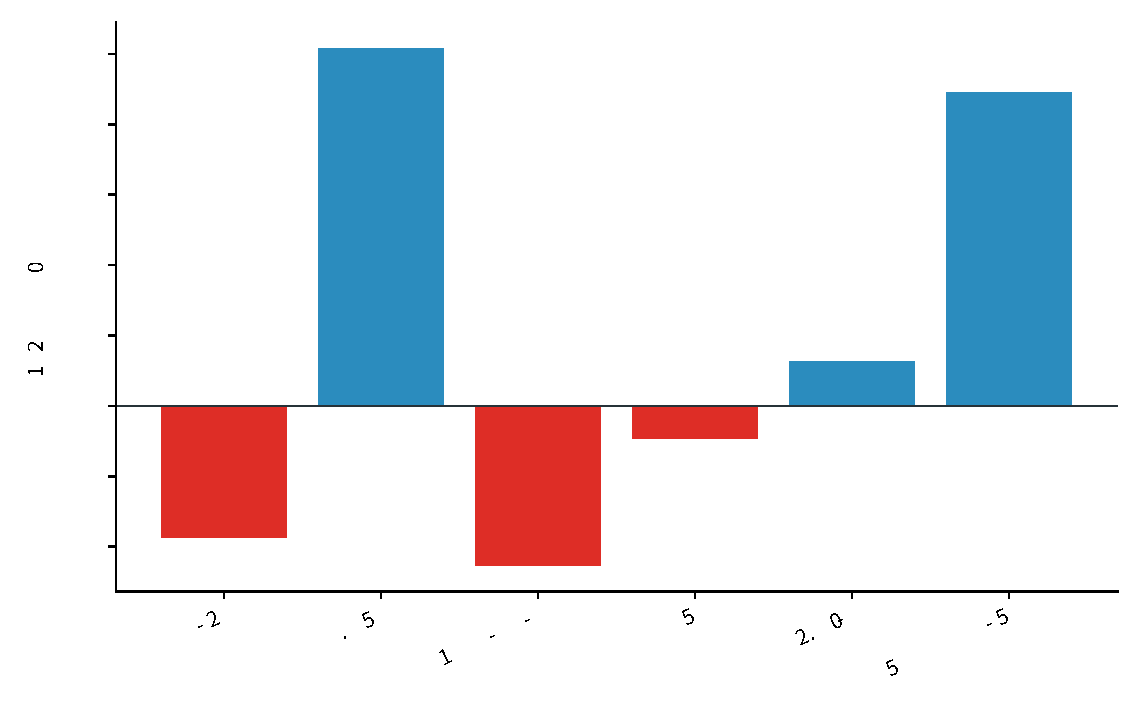
\includegraphics[width=\linewidth]{figures/per_class_evidence_gain.pdf}
  \caption{不同证据配置的逐类别候选判断增益}
  \label{fig:per_class_evidence_gain}
\end{figure}

\subsection{RQ2：端到端纠错}
\label{subsec:rq2}

RQ2比较八种端到端设置。B0以0.001低阈值保留完整检测排序，只用于mAP参考。B1是验证集选择的检测器工作点。B2只使用ECC、SSIM、形态学差异候选和冻结拓扑规则，不调用验证器。B7对抽样候选全量复核且不使用门控，B8采用手工线性风险门。Full采用学习式Logistic复检门、分动作接受门和安全规则。Oracle-C在完整固定候选集上按真值选择最优动作，反映候选覆盖上界。Oracle-A只在已有真实验证器输出的候选中接受正效用动作，反映当前提议动作集合的接受上界。

五折固定候选共51222个，超过既定调用上限。实验在每折按原始错误类型和候选来源比例分层抽样800个候选，共评价约4000个候选。未抽中的候选保持B1输出。抽样比例从fold\_0的5.5348\%到fold\_4的12.5156\%。所有方法共享同一批A2响应，B7、B8和Full之间的差异来自门控而非调用样本变化。表~\ref{tab:rq2_main}报告五折均值与折间标准差。

\begin{table*}[t]
  \centering
  \caption{RQ2五折端到端结果}
  \label{tab:rq2_main}
  \setlength{\tabcolsep}{5pt}
  \begin{tabular}{lcccc}
    \hline
    方法 & F1 & mAP@0.5 & TPRR & HCR \\
    \hline
    B0$^{\dagger}$ & $0.2871\pm0.0813$ & $0.9491\pm0.0205$ & 不适用 & 不适用 \\
    B1 & $0.9118\pm0.0344$ & $0.8813\pm0.0575$ & 不适用 & 不适用 \\
    B2 & $0.0014\pm0.0011$ & $0.0001\pm0.0002$ & 不适用 & 不适用 \\
    B7 & $0.8660\pm0.0368$ & $0.8246\pm0.0655$ & $0.9572\pm0.0174$ & $0.9326\pm0.0280$ \\
    B8 & $0.8787\pm0.0471$ & $0.8450\pm0.0867$ & $0.9717\pm0.0305$ & $0.9607\pm0.0456$ \\
    Full & $0.9117\pm0.0343$ & $0.8810\pm0.0573$ & $0.9998\pm0.0003$ & $0.4000\pm0.5477$ \\
    Oracle-C & $0.9555\pm0.0254$ & $0.9106\pm0.0471$ & 不适用 & 不适用 \\
    Oracle-A & $0.9143\pm0.0336$ & $0.8826\pm0.0573$ & $1.0000\pm0.0000$ & $0.0000\pm0.0000$ \\
    \hline
  \end{tabular}
  \vspace{2pt}
  \parbox{0.95\textwidth}{\footnotesize $^{\dagger}$B0使用0.001低阈值保留检测排序，其F1只描述该阈值下的输出，不作为部署工作点结论。}
\end{table*}

B2的F1只有0.0014，说明确定性差异规则不能单独替代检测器。无门控B7把F1从B1的0.9118降至0.8660，HCR达到0.9326。绝大多数已执行修改降低了检测效用。手工线性门B8的F1为0.8787，仍低于B1，HCR为0.9607。缺少动作级安全约束时，验证器输出不能作为可靠的后置纠错结果。

Full的F1为$0.9117\pm0.0343$，B1为$0.9118\pm0.0344$。按图像聚类的配对bootstrap给出总体F1差值$-0.000064$。95\%置信区间为$[-0.000273,+0.000094]$，区间跨越0。Full与B1无统计差异，完整流程未获得可辨别的端到端净提升。小数点后的波动不能表述为性能改进。Full的TPRR达到0.9998，学习式双门控基本保留了原始正确检测。HCR均值为0.4000，折间标准差为0.5477。实际接受动作很少，个别折的一次有害动作会使该折比率大幅变化。因此，安全性需要结合绝对动作计数解释。

图~\ref{fig:error_transfer}和表~\ref{tab:error_transfer}给出错误转移。约4000个评价候选中，48个原始误报只纠正1个，47个未纠正。36个漏检均未恢复，6个错分类均未修正。734个原始正确检测中，732个保持正确，2个被误删。3174个差异噪声候选和2个纯定位错误也均未纠正。Full未发生误改类别、差异候选新增误报或将错误类别改成另一错误类别，实际损失均来自2次误删TP。双门控大幅减少了有害修改，但几乎没有放行有效修正。

\begin{table}[t]
  \centering
  \caption{Full候选级错误转移计数}
  \label{tab:error_transfer}
  \setlength{\tabcolsep}{4pt}
  \begin{tabular}{lrrrr}
    \hline
    原始类型 & 保持正确 & 已纠正 & 未纠正 & 误删 \\
    \hline
    误报 & 0 & 1 & 47 & 0 \\
    漏检 & 0 & 0 & 36 & 0 \\
    错分类 & 0 & 0 & 6 & 0 \\
    正确检测 & 732 & 0 & 0 & 2 \\
    \hline
  \end{tabular}
\end{table}

\begin{figure}[t]
  \centering
  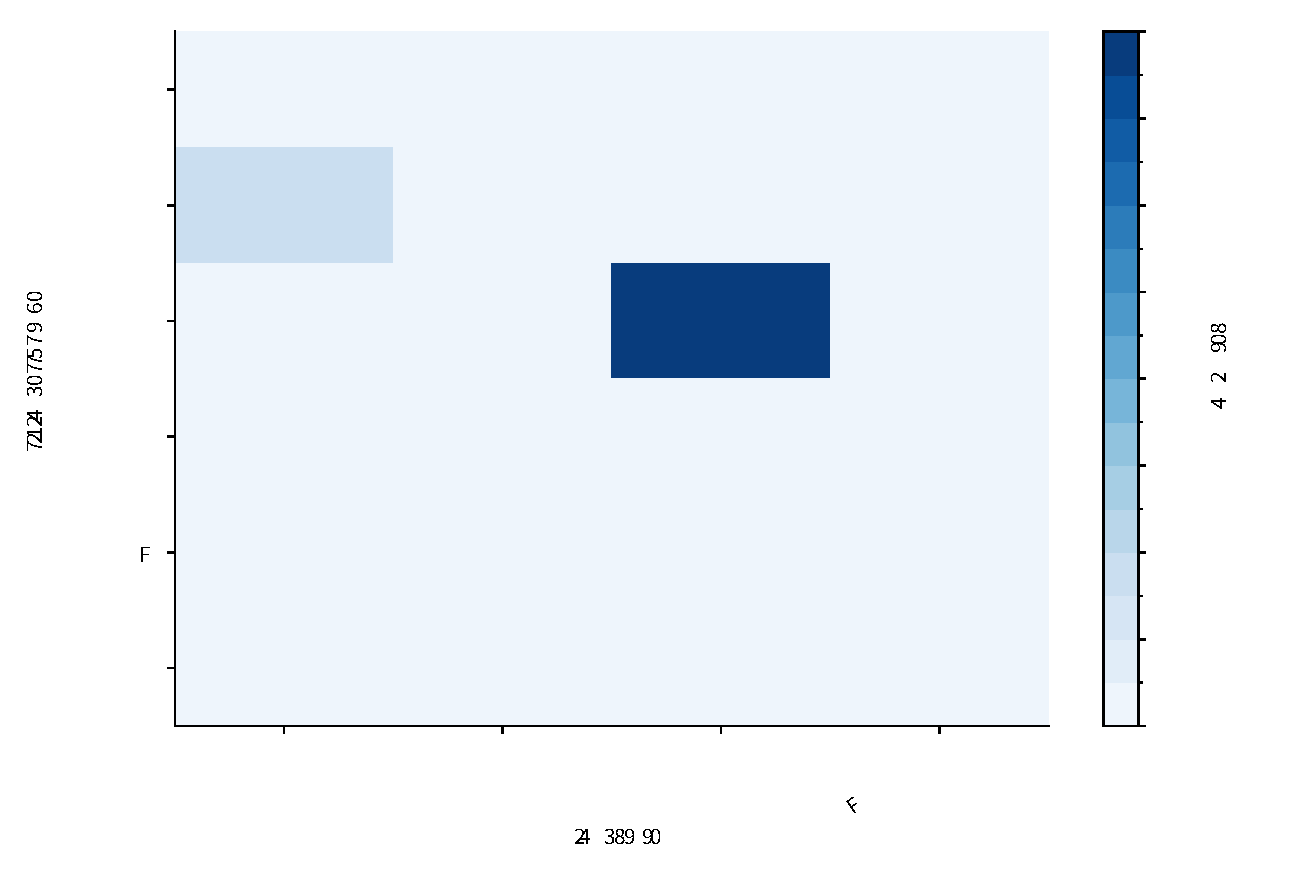
\includegraphics[width=\linewidth]{figures/error_transfer_heatmap.pdf}
  \caption{Full方法的候选级错误转移热图}
  \label{fig:error_transfer}
\end{figure}

Oracle结果用于定位限制因素。Oracle-C的F1为0.9555，相对B1保留约0.044的提升空间，说明固定候选集仍有纠错潜力。Oracle-A只接受真实验证器输出中的正效用动作，F1也仅为0.9143，相对B1提高0.0025。即使接受决策达到理想状态，当前提议动作仍远未达到候选上界。B1与Oracle-C之间的大部分空间损失在验证器判断阶段，而非复检门或接受门。RQ2表明双门控大幅减少了有害修改，但端到端净收益接近零。当前主要限制因素是多模态验证器对工业细粒度缺陷的判断质量。

\subsection{RQ3：门控效率与可靠性}
\label{subsec:rq3}

RQ3在RQ2的同一批A2缓存上离线回放六种策略和六个预算点。预算是每折800个抽样候选中的调用比例，取5\%、10\%、20\%、40\%、60\%和100\%。random按固定随机种子抽样，low\_confidence按检测置信度排序。manual\_linear使用手工线性风险分数。logistic和lightgbm使用学习式复检分数排序。review\_acceptance在logistic排序后执行接受门与安全规则。表~\ref{tab:rq3_budget}列出全部36个组合的五折均值，RR表示错误候选复核召回率。

\begin{table*}[t]
  \centering
  \caption{六种门控策略在六个调用预算下的结果，数值为五折均值}
  \label{tab:rq3_budget}
  \setlength{\tabcolsep}{3.5pt}
  \begin{tabular}{llrrrrrr}
    \hline
    策略 & 指标 & 5\% & 10\% & 20\% & 40\% & 60\% & 100\% \\
    \hline
    random & F1 & 0.9088 & 0.9067 & 0.9015 & 0.8915 & 0.8820 & 0.8660 \\
           & HCR & 0.9633 & 0.9471 & 0.9342 & 0.9382 & 0.9335 & 0.9326 \\
           & RR & 0.0315 & 0.1322 & 0.2251 & 0.3951 & 0.5763 & 1.0000 \\
    \hline
    low\_confidence & F1 & 0.9116 & 0.9112 & 0.9096 & 0.9055 & 0.9013 & 0.8660 \\
           & HCR & 0.6000 & 0.8000 & 1.0000 & 1.0000 & 0.9935 & 0.9326 \\
           & RR & 0.0000 & 0.0000 & 0.0065 & 0.0769 & 0.2048 & 1.0000 \\
    \hline
    manual\_linear & F1 & 0.9106 & 0.9096 & 0.9077 & 0.9032 & 0.8989 & 0.8660 \\
           & HCR & 1.0000 & 1.0000 & 0.9913 & 0.9913 & 0.9812 & 0.9326 \\
           & RR & 0.0129 & 0.0614 & 0.1644 & 0.2820 & 0.4614 & 1.0000 \\
    \hline
    logistic & F1 & 0.9076 & 0.9006 & 0.8942 & 0.8856 & 0.8782 & 0.8660 \\
           & HCR & 0.6813 & 0.8059 & 0.8697 & 0.8977 & 0.9156 & 0.9326 \\
           & RR & 0.4649 & 0.5103 & 0.6686 & 0.8397 & 0.9347 & 1.0000 \\
    \hline
    lightgbm & F1 & 0.9094 & 0.9050 & 0.8966 & 0.8838 & 0.8744 & 0.8660 \\
           & HCR & 0.6597 & 0.7708 & 0.8452 & 0.8960 & 0.9158 & 0.9326 \\
           & RR & 0.6236 & 0.7455 & 0.8562 & 0.9230 & 0.9700 & 1.0000 \\
    \hline
    review\_acceptance & F1 & 0.9117 & 0.9116 & 0.9115 & 0.9115 & 0.9115 & 0.9115 \\
           & HCR & 0.4000 & 0.4000 & 0.4000 & 0.4000 & 0.4000 & 0.4000 \\
           & RR & 0.4649 & 0.5103 & 0.6686 & 0.8397 & 0.9347 & 1.0000 \\
    \hline
  \end{tabular}
\end{table*}

复检门的排序效率在低预算区间最清楚。5\%预算下，Logistic复检门覆盖46.49\%的错误候选，随机策略仅覆盖3.15\%，前者约为后者的14.8倍。LightGBM在同一预算达到62.36\%。其PR AP为0.4311，高于Logistic的0.1839。端到端实验按预注册协议固定使用Logistic主模型，未依据测试结果更换。低置信度策略在5\%和10\%预算下的错误候选复核召回均为0。检测置信度不能替代针对“是否值得复核”训练的风险分数。复检门将有限调用集中到潜在可纠错位置，但不保证验证器修改正确。

接受门决定预算扩大后是否退化。不使用接受门时，随机回放的F1从5\%预算的0.9088降至100\%预算的0.8660，累计下降0.0428。20\%和60\%预算下分别为0.9015和0.8820。加入接受门后，F1从5\%预算的0.9117变为20\%、60\%和100\%预算下约0.9115。各预算结果与B1无统计差异，保持在基线水平。该稳定性来自多数提议未被执行，不代表验证器判断改善。HCR维持0.4000仍需结合RQ2中的极少接受动作解释，不能作为充分校准的概率保证。

调用成本随预算近似线性增加。六种策略在相同预算下调用数一致。每图调用次数从5\%预算的$0.1341\pm0.0118$增至100\%预算的$2.6821\pm0.2363$。真实缓存记录给出的单候选平均时延约29.1秒，跨策略与预算的P95最高约41.4秒。每图输入token数在logistic的5\%预算下为$123.35\pm10.64$。该数值在100\%预算下增至$2518.81\pm223.24$。在当前后端吞吐下，全量复核会降低F1并增加调用成本。低预算复检门控制调用量，接受门控制动作风险。

图~\ref{fig:rq3_curves}给出F1、HCR与调用率曲线。图~\ref{fig:acceptance_reliability}给出接受门可靠性分析。可靠性图的横轴为预测概率，纵轴为观测正效用率。曲线多处偏离理想对角线，与抽样动作上的校准不稳定一致。门控曲线显示复检门提高错误覆盖效率，接受门控制已执行动作的风险。只有复检门时，高风险候选更快进入复核，但错误提议仍使F1下降。只有接受门时，系统能减少有害修改，却不能降低验证器调用成本。因此，两道门承担不同任务。

\begin{figure*}[t]
  \centering
  \begin{minipage}{0.48\textwidth}
    \centering
    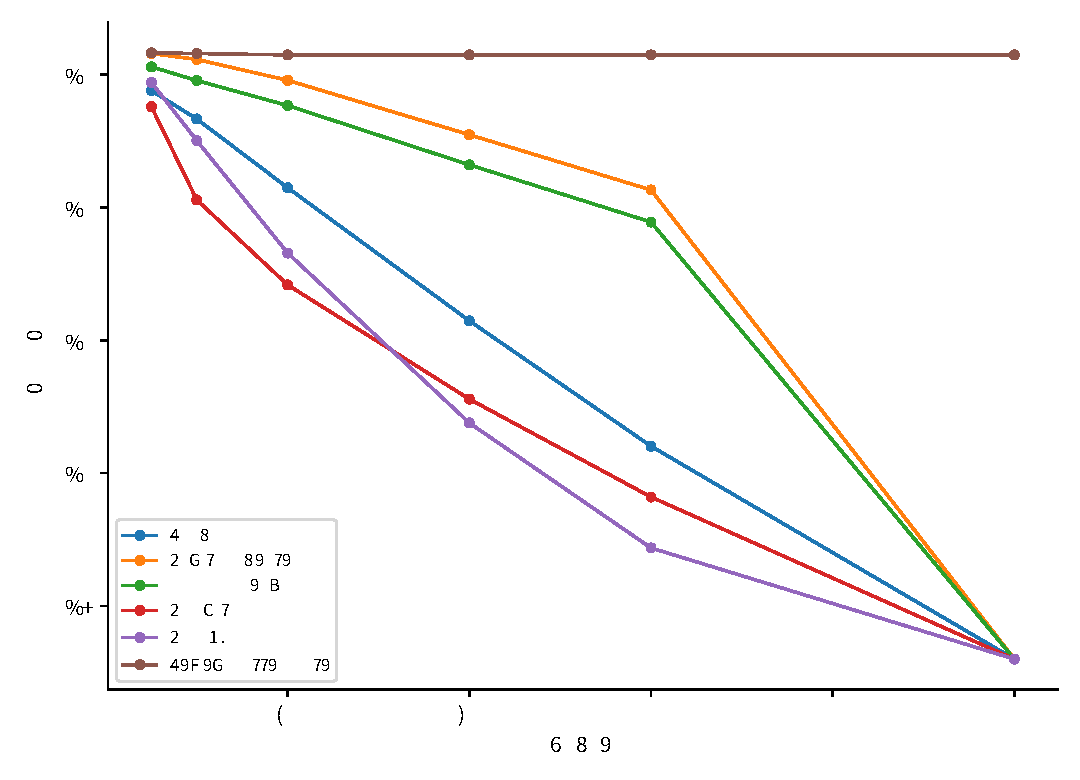
\includegraphics[width=\linewidth]{figures/f1_call_rate.pdf}
    \small (a) F1与调用率
  \end{minipage}\hfill
  \begin{minipage}{0.48\textwidth}
    \centering
    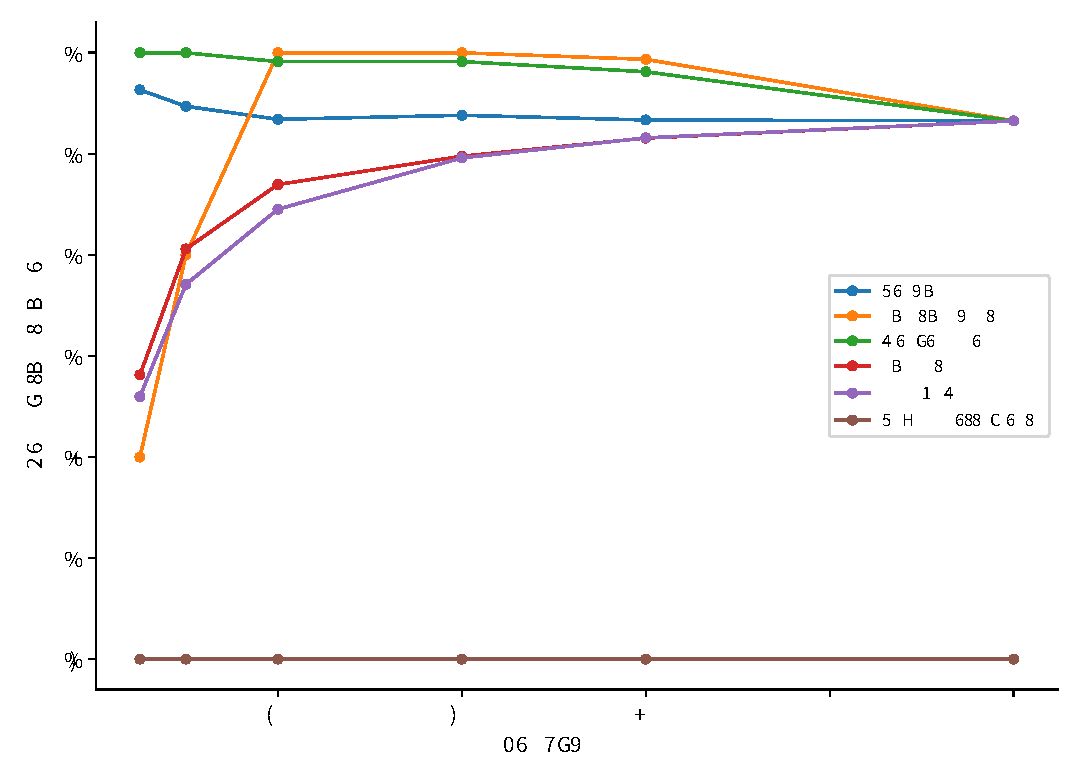
\includegraphics[width=\linewidth]{figures/hcr_call_rate.pdf}
    \small (b) HCR与调用率
  \end{minipage}
  \caption{不同门控策略的性能、风险与调用预算关系}
  \label{fig:rq3_curves}
\end{figure*}

\begin{figure}[t]
  \centering
  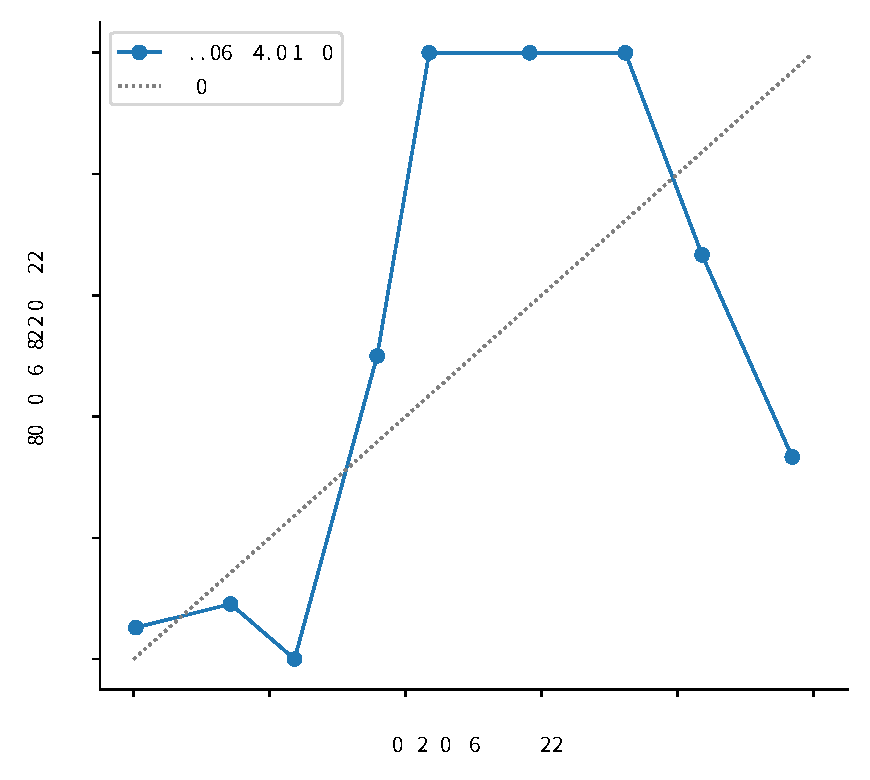
\includegraphics[width=\linewidth]{figures/acceptance_reliability.pdf}
  \caption{接受门的可靠性分析}
  \label{fig:acceptance_reliability}
\end{figure}

\subsection{RQ4：鲁棒性与模型替换}
\label{subsec:rq4}

RQ4在fold\_0的325张测试图像上进行。几何扰动施加于正常模板，光度扰动施加于待检图。每个条件重新计算配准、光度归一、外观残差、骨架差异和差异候选。几何实验组合无二次配准或ECC配准、直接XOR或容差XOR，以及是否使用配准质量阈值。这些组合共产生8775条图像与扰动条件评价记录。fold\_0共有343个基础漏检。漏检恢复率以完整测试折为分母，定义为差异候选与未覆盖真值框达到IoU不低于0.3的比例。最终F1和HCR使用fold\_0的800个真实A2结论冻结回放，只重算扰动影响的证据与门控特征。该协议隔离了配准证据退化，但不等价于在每种扰动下重新调用验证器。

\subsubsection{容差XOR与配准质量}

无额外扰动时，ECC加直接XOR恢复23个漏检，恢复率为$23/343=6.71\%$。改用容差XOR后恢复81个，达到$81/343=23.62\%$，提升约3.5倍。XOR伪差异像素占比同时从0.02892降至0.01441，降低约50\%。容差操作允许骨架在小邻域内匹配，从而压制JPEG边缘和亚像素错位产生的双边轮廓。表~\ref{tab:rq4_xor}表明，恢复率提高并未增加伪差异面积。

\begin{table}[t]
  \centering
  \caption{无额外扰动时直接XOR与容差XOR比较}
  \label{tab:rq4_xor}
  \setlength{\tabcolsep}{4pt}
  \begin{tabular}{lrr}
    \hline
    设置 & 漏检恢复率 & XOR占比 \\
    \hline
    ECC+直接XOR & 23/343=6.71\% & 0.02892 \\
    ECC+容差XOR & 81/343=23.62\% & 0.01441 \\
    \hline
  \end{tabular}
\end{table}

在同方向正平移序列中，$q_{\mathrm{reg}}$均值随扰动增大而下降。无扰动、平移2像素和平移8像素时，均值分别为0.8599、0.8410和0.7992。对应$q_{\mathrm{reg}}<0.5$的比例为4.00\%、4.62\%和4.92\%。该受控序列说明质量分能响应逐渐增强的错位。平移8像素时，完整设置的F1为0.8796，HCR为1.0000。相关强扰动条件只有1个被接受动作，且该动作有害。HCR为1不表示大量候选受到破坏，只说明这一次放行动作失败。

配准质量阈值的保护作用未获实证。全部几何条件中，冻结阈值0.5没有拦截任何有害动作，因为相关候选的$q_{\mathrm{reg}}$均未低于阈值。$q_{\mathrm{reg}}$同时惩罚估计变换幅度。ECC修正真实初始错位后，其分数有时低于以恒等变换计算的代理分数。本实验只支持$q_{\mathrm{reg}}$在选定平移强度序列中的下降趋势，不支持它在所有几何扰动间严格单调。当前阈值也未形成可靠的风险保证。该负面结果与容差XOR的收益属于不同结论。

光度扰动包括亮度$\pm10$、$\pm20$，对比度0.8和1.2，两档噪声以及两档模糊。完整设置在这些条件下的最终F1均为0.8803，HCR均为0。DeepPCB像素主要集中在0和255附近，较小光度变化的区分度有限。该结果只说明冻结回放协议下没有触发额外有害修改，不能推广为对任意成像变化鲁棒。图~\ref{fig:rq4_registration}汇总了XOR表示、配准质量分布和配准扰动性能。

\begin{figure*}[t]
  \centering
  \begin{minipage}{0.32\textwidth}
    \centering
    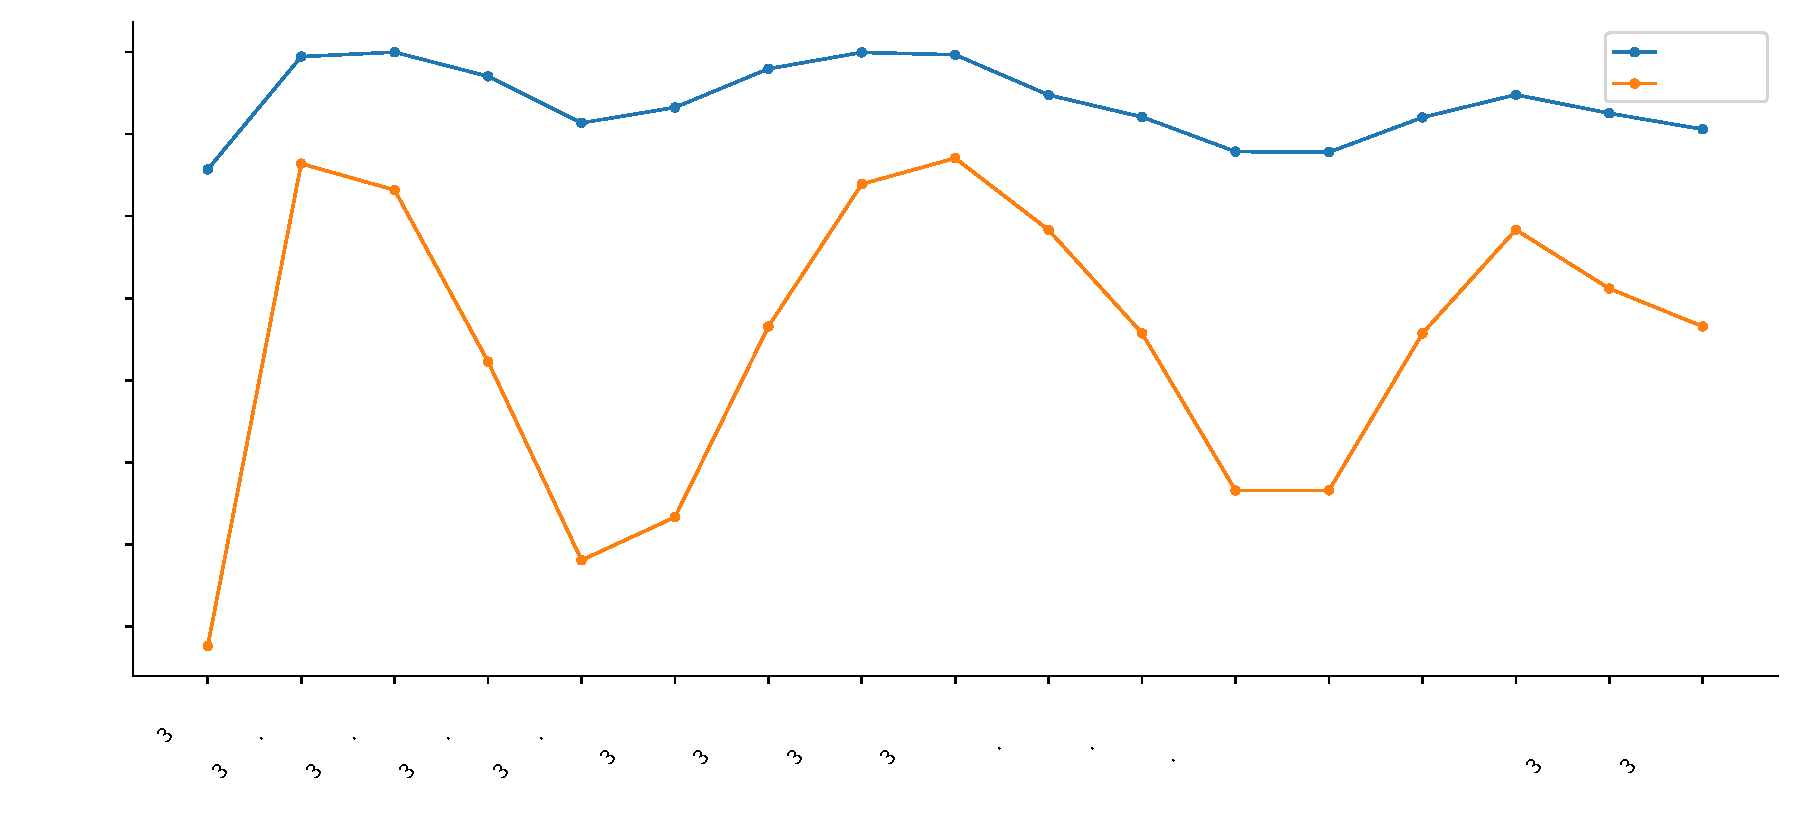
\includegraphics[width=\linewidth]{figures/rq4_xor_comparison.pdf}
    \small (a) XOR表示比较
  \end{minipage}\hfill
  \begin{minipage}{0.32\textwidth}
    \centering
    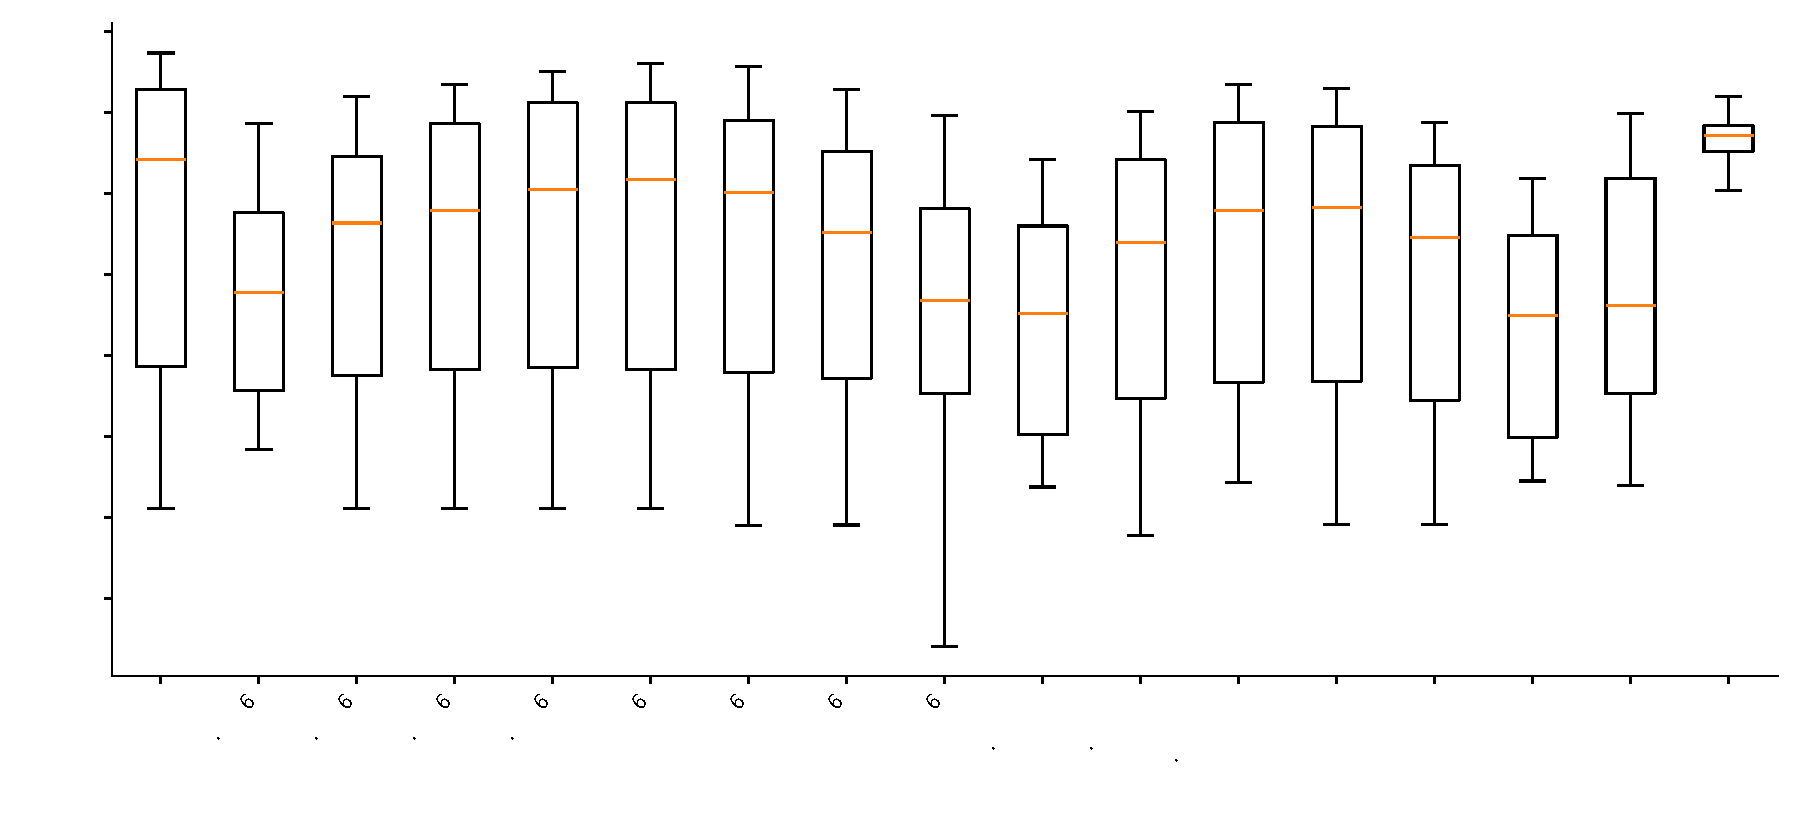
\includegraphics[width=\linewidth]{figures/rq4_qreg_distribution.pdf}
    \small (b) 配准质量分布
  \end{minipage}\hfill
  \begin{minipage}{0.32\textwidth}
    \centering
    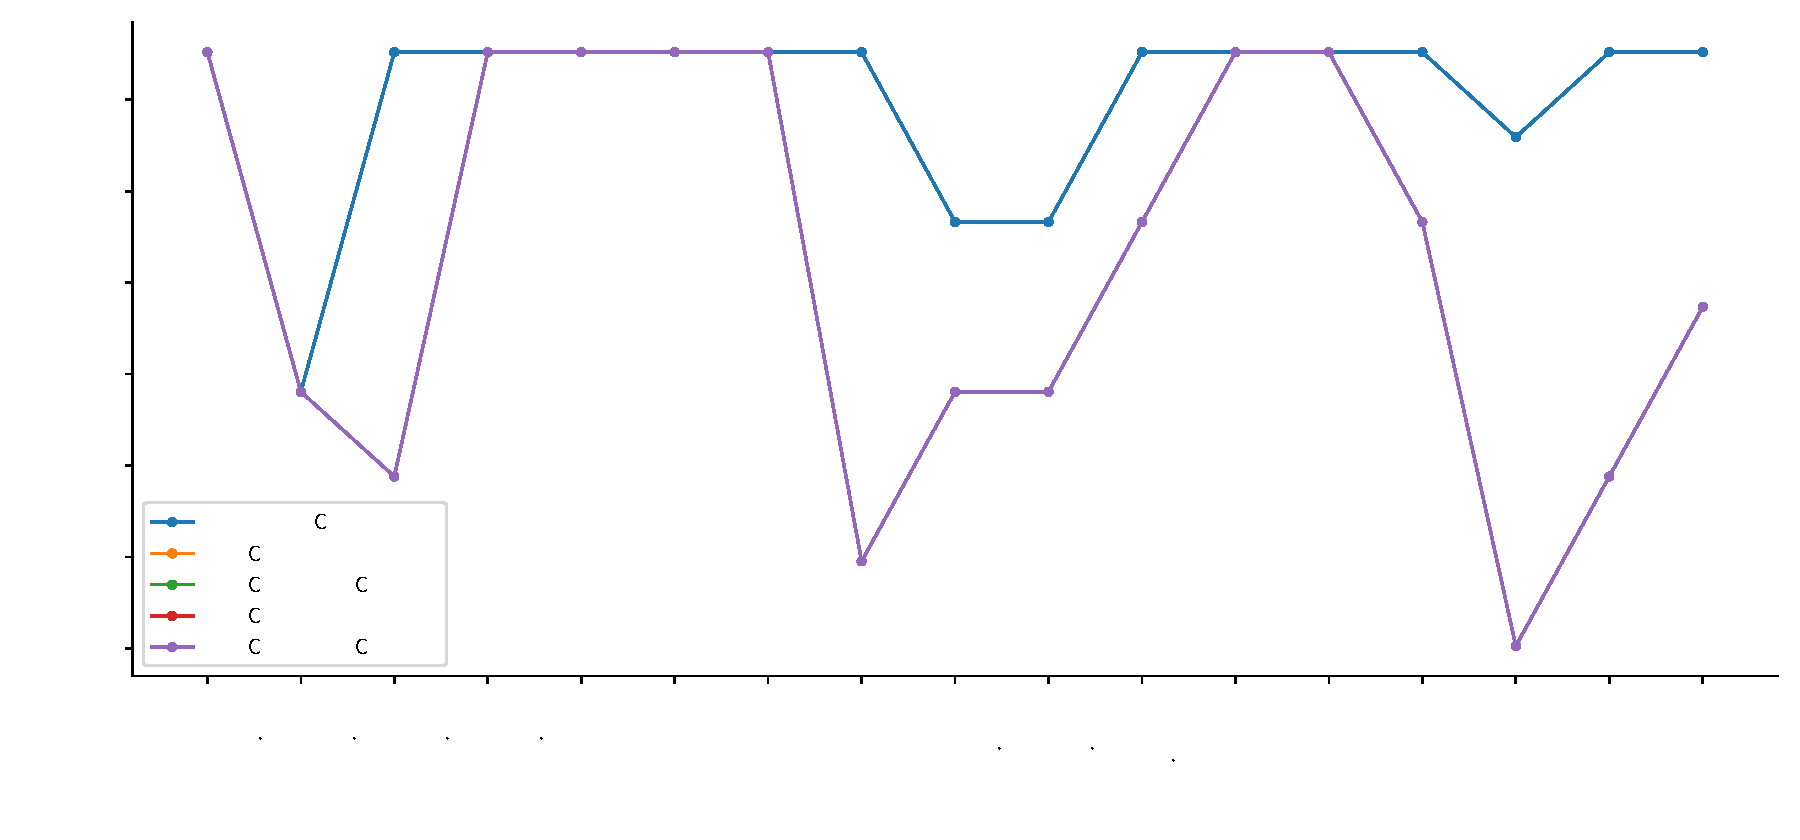
\includegraphics[width=\linewidth]{figures/rq4_registration_performance.pdf}
    \small (c) 配准扰动性能
  \end{minipage}
  \caption{配准扰动、质量分与容差XOR的鲁棒性结果}
  \label{fig:rq4_registration}
\end{figure*}

\subsubsection{检测器与门控模型替换}

检测器替换采用官方PekingU RT-DETR-R18VD。模型在fold\_0训练后预测全部测试图像，并对200个比例分层候选调用A2验证器。表~\ref{tab:rq4_model}显示，RT-DETR-R18VD基线F1为0.6416，mAP@0.5为0.6483。二者均低于YOLOv8s五折工作点。完整流程实际调用12次，但没有接受任何修改。最终F1仍为0.6416，HCR为0。该对照没有出现性能退化。由于系统未执行动作，结果不能证明双门控在检测器替换时有效，也不能证明流程能改善不同架构的检测性能。

门控模型替换也限制在fold\_0的200个分层候选上。Logistic在验证阈值0.208300下调用0次。LightGBM在阈值0.145905下调用3次。两者最终F1均为0.8803，HCR均为0。调用数过少，无法比较两种模型的纠错能力，也不足以验证安全规则对门控分类器变化的稳健性。

\begin{table}[t]
  \centering
  \caption{RQ4检测器替换结果}
  \label{tab:rq4_model}
  \setlength{\tabcolsep}{4pt}
  \begin{tabular}{lrrr}
    \hline
    设置 & F1 & mAP@0.5 & HCR \\
    \hline
    RT-DETR-R18VD基线 & 0.6416 & 0.6483 & 不适用 \\
    RT-DETR-R18VD+完整流程 & 0.6416 & 0.6483 & 0.0000 \\
    \hline
  \end{tabular}
\end{table}

第二个多模态验证器后端未完成对照，HRIPCB也未纳入实验。RQ4支持的确定性发现是：容差XOR在DeepPCB fold\_0上提高漏检候选恢复率，并减少伪差异。RT-DETR-R18VD对照中没有接受任何修改，因而只能报告未发生有害动作。跨检测器增益、跨数据集泛化和跨验证器一致性均超出当前证据范围。

\subsection{讨论与局限}
\label{subsec:discussion_limitations}

四个研究问题给出一致的能力边界。正常模板提高了验证器的候选存在性判断，完整外观与拓扑证据没有稳定增量。双来源候选保留了Oracle-C上界，真实验证器输出对应的Oracle-A增益只有0.0025。复检门能在低预算下集中覆盖错误候选，接受门使各预算结果与基线无统计差异。端到端Full仍未超过基础工作点。当前实验支持风险受控的复核流程，不支持稳定提高检测指标的结论。以下四项局限限定了结论范围。

第一项局限是接受门的训练分布与部署提议分布不完全匹配。训练阶段的remove、relabel和add提议由冻结的确定性证据代理生成，正效用标签由折外检测和真值计算。端到端部署的提议则来自真实验证器。两类提议的类别频率、错误模式和分数分布存在差异风险，可能造成接受概率失配。该问题直接影响HCR、动作召回和阈值可靠性，也能解释接受门过度保守以及Oracle-A高于Full的部分差距。它不影响YOLOv8s基础检测指标、RQ1的证据输入比较和Oracle-C候选覆盖结论。后续实验需使用已积累的约7000次真实调用重训接受门，并在独立模板组上重新校准阈值。

第二项局限是实验只有一个真实多模态验证器后端。RQ1的证据偏好、自由文本解析失败、标签可见对照和RQ2的Oracle-A上限均基于\texttt{gpt-5.6-sol}。当前结果只支持“该后端在本协议下判断质量不足”，不能推广到所有视觉语言模型。检测器替换不能弥补这一缺口，因为验证器保持不变。该局限影响所有涉及验证器正确率和提示行为的结论。数据泄漏判断、基础错误分解、容差XOR的确定性候选结果和调用成本实测不受此限制。

第三项局限来自RQ2的分层抽样评价。五折固定候选总数为51222，每折只调用800个，覆盖比例为5.5\%至12.5\%。未抽中的候选保持B1输出。该协议能在调用预算内公平比较B7、B8和Full，也能精确计数抽样区域内的错误转移。大量未修改候选会稀释端到端净收益，稀有正确动作也可能未进入样本。Full相对B1的bootstrap区间只描述本抽样与冻结响应协议，不等于全量调用51222个候选后的区间。Oracle-C使用完整固定候选集，仍可判断候选覆盖潜力。Oracle-A、FPCR、MDRR、MCCA和错误转移矩阵均受抽样范围约束。

第四项局限是fold\_0测试集只包含group20085一个模板组。该折有325对图像，样本量最大，但板型多样性最低。RQ4主要在该折执行，其扰动结果会受到单一模板结构特征的影响。五折总体检测与RQ2主表仍覆盖全部11个模板组。fold\_0的单组性质主要限制RQ4配准趋势、RT-DETR替换和门控替换的外推范围。后续实验需在其余四折重复关键扰动，并按模板组汇总$q_{\mathrm{reg}}$和漏检恢复率。这些实验将检验容差XOR收益是否为group20085特有现象。

官方划分存在模板泄漏，按模板组隔离是主结论成立的前提。正常模板和学习式复检排序分别获得证据消融与低预算覆盖率的支持。接受门使各预算结果保持在基线水平，但Full的HCR仍为0.4000，并有2次误删TP。完整证据卡与去锚定协议没有显示稳定优势。Oracle-C与Oracle-A的差距表明，当前主要限制因素是验证器判断质量。Full与B1无统计差异，端到端净收益接近零。

\section{总结与展望}
\label{sec:conclusion}

\subsection{工作总结}

本文研究正常模板可用条件下的PCB检测结果复核，并构建由候选生成、多模态验证器、复检门和接受门组成的后置系统。实验同时给出有效组件、无显著增量的设计和端到端能力边界。

系统合并基础检测候选与差异候选，使复核范围不受基础检测器输出限制。阶段A调参后，差异候选在IoU 0.3下的漏检恢复率达到0.625。Oracle-C的F1为0.9555，相对基础方法保留约0.044的纠错空间。双来源候选覆盖了一部分基础检测器未提出的位置，但候选覆盖不等同于端到端纠错收益。

系统使用配准质量、检测不确定性和候选来源进行分级复核。在5\%调用预算下，Logistic复检门覆盖46.49\%的可纠错错误，随机选择覆盖3.15\%，前者约为后者的14.8倍。$q_{\mathrm{reg}}$在选定的同方向平移序列中随扰动增强而下降，可作为配准可靠性指标。强扰动条件下的HCR为1.0，但分母只有1个被接受动作。冻结阈值0.5的配准质量规则没有拦截任何有害动作。因此，当前实验尚未验证该规则的保护作用，也不支持质量分在所有几何扰动间严格单调。

学习式接受门和硬安全规则约束验证器动作。完整系统的正确检测保留率为0.9998，734个正确检测中误删2个。双门控将HCR从无门控全量复核的0.9326降至0.4000，并把误删控制在2次，仍有有害修改发生。加入接受门后，各调用预算下的F1与B1无统计差异，保持在基线水平。该结果支持双门控大幅减少有害修改，不能解释为系统消除了动作风险。

显式外观差异图与拓扑图没有形成预期贡献。200候选主消融中，A4为0.7571，略高于A2的0.7553，但差异处于置信区间内，未证明拓扑图带来增量。A5和A6相对A0的置信区间均跨零，因此不显著。阶段B2的450次专门对照采用另一批150个候选，A2为0.8082，并高于全部含差异图的变体。两个实验口径不能混用。最终系统移除显式差异视觉输入，只保留拓扑统计作为门控特征。去锚定设计也未获支持，提供检测标签的对照更好。

\subsection{结论与能力边界}

双门控大幅减少了有害修改，但端到端净收益接近零。五折实验中，完整系统F1为$0.9117\pm0.0343$，基础方法为$0.9118\pm0.0344$。二者的配对bootstrap差值为$-0.000064$，95\%置信区间为$[-0.000273,+0.000094]$，区间跨零。完整系统mAP@0.5为0.8810，基础方法为0.8813。当前证据不支持“复核系统提升整体检测精度”的结论。

Oracle分析进一步定位了限制因素。Oracle-C的F1为0.9555，说明候选集合仍有纠错空间。即使接受门理想地选择当前验证器提出的动作，Oracle-A的F1也只有0.9143，仅比基础方法高0.0025。当前主要限制因素是验证器对工业细粒度缺陷的判断和动作提议质量，而非候选覆盖。实验支持复检门提高有限预算下的错误候选覆盖效率，也支持接受门减少有害修改。实验不支持整体精度提升，端到端净收益接近零。

\subsection{未来工作}

接受门需要匹配真实提议分布。现有接受门使用确定性证据代理产生的动作训练，实验已积累约7000次真实验证器调用及其缓存输出。后续可据此重建动作级训练集，并按模板组隔离训练与测试。新模型仍需以正确检测保留率和有害修正率作为硬约束。

跨后端验证需要至少一个独立的多模态验证器，并在相同候选、证据卡、提示和预算下进行配对比较。跨模型一致的失败可用于检查任务或证据设计。模型间差异可用于分析领域能力、校准和动作偏好。当前单一后端的结论不能泛化到全部多模态验证器。

跨数据集实验可在HRIPCB上按模板分组，避免同一模板跨训练集与测试集造成泄漏。评价需分别报告配准成功率、差异候选召回、门控覆盖率与最终检测指标。该实验用于检验当前DeepPCB结果能否迁移到旋转变化和更多模板条件。

端到端增益取决于工业细粒度缺陷的领域适配。候选级正常与缺陷图对、缺陷类别知识和真实纠错动作可用于监督微调或偏好优化，第二模型或外部视觉专家可提供对照反馈。领域适配后的验证器仍需经过独立接受门，模型能力不能替代系统安全约束。


\bibliographystyle{IEEEtran}
\bibliography{refs}

\end{document}
